% ============================================================
% Semester Project — Deepspace Defenders
% Object Oriented Programming Techniques (CSE142)
% Institute of Business Administration Karachi
% ============================================================

\documentclass[11pt]{article}

% ── Packages ──────────────────────────────────────────────────────────────
\usepackage[a4paper, margin=1in]{geometry}
\usepackage[utf8]{inputenc}
\usepackage[T1]{fontenc}
\usepackage{amsmath, amssymb, amsthm}
\usepackage{graphicx}
\usepackage{hyperref}
\usepackage{listings}
\usepackage{xcolor}
\usepackage{titlesec}
\usepackage{fancyhdr}
\usepackage{parskip}
\usepackage{caption}
\usepackage{subcaption}
\usepackage{booktabs}
\usepackage{array}
\usepackage{enumitem}
\usepackage{float}
\usepackage{tikz}
\usepackage{tcolorbox}
\tcbuselibrary{skins,breakable}
\usetikzlibrary{shapes,arrows,positioning,fit,backgrounds,calc}

% ── Colours ───────────────────────────────────────────────────────────────
\definecolor{primary}{RGB}{165, 28, 48}
\definecolor{secondary}{RGB}{0, 53, 107}
\definecolor{accent}{RGB}{232, 95, 26}
\definecolor{codebg}{RGB}{245, 248, 250}
\definecolor{codecomment}{RGB}{106, 153, 85}
\definecolor{codekeyword}{RGB}{0, 0, 200}
\definecolor{codestring}{RGB}{163, 21, 21}
\definecolor{stdtype}{RGB}{43, 145, 175}

% ── C++ Listing style ─────────────────────────────────────────────────────
\lstdefinestyle{cpp}{
    language=C++,
    backgroundcolor=\color{codebg},
    basicstyle=\ttfamily\small,
    breaklines=true,
    captionpos=b,
    commentstyle=\color{codecomment}\itshape,
    keywordstyle=\color{codekeyword}\bfseries,
    stringstyle=\color{codestring},
    numbers=left,
    numbersep=8pt,
    numberstyle=\tiny\color{gray},
    frame=single,
    rulecolor=\color{gray!40},
    showstringspaces=false,
    tabsize=4,
    xleftmargin=1.5em,
    framexleftmargin=1.5em,
    morekeywords={override, nullptr, auto, decltype, noexcept,
                  final, constexpr, explicit, virtual, class, struct,
                  public, private, protected, new, delete, this},
}
\lstset{style=cpp}

% ── Header / Footer ───────────────────────────────────────────────────────
\pagestyle{fancy}
\fancyhf{}
\renewcommand{\headrulewidth}{0.4pt}
\fancyhead[L]{\textcolor{primary}{\textbf{\mytitle}}}
\fancyhead[R]{\textcolor{primary}{\thepage}}

\fancypagestyle{firstpage}{
    \fancyhf{}
    \renewcommand{\headrulewidth}{0pt}
    \fancyfoot[C]{\textcolor{gray}{\small \mytitle\ -- \thepage}}
}

% ── Section formatting ────────────────────────────────────────────────────
\titleformat{\section}
    {\normalfont\Large\bfseries\color{primary}}{\thesection}{1em}{}
\titleformat{\subsection}
    {\normalfont\large\bfseries\color{secondary}}{\thesubsection}{1em}{}
\titleformat{\subsubsection}
    {\normalfont\normalsize\bfseries\color{accent}}{\thesubsubsection}{1em}{}

% ── TikZ node styles ──────────────────────────────────────────────────────
\tikzset{
    block/.style={rectangle, draw=secondary, fill=blue!8, text width=2.8cm,
                  text centered, rounded corners, minimum height=1cm, font=\small},
    abstract/.style={rectangle, draw=primary, fill=primary!10, text width=2.8cm,
                  text centered, rounded corners, minimum height=1cm,
                  font=\small\itshape},
    struct/.style={rectangle, draw=accent, fill=accent!8, text width=2.4cm,
                  text centered, rounded corners, minimum height=0.9cm, font=\small},
    line/.style={draw, -latex, thick},
    dashed_line/.style={draw, dashed, -latex},
}

% ── Info boxes ────────────────────────────────────────────────────────────
\newtcolorbox{infobox}{
    colback=primary!5, colframe=primary, boxrule=0.6pt,
    arc=3pt, left=8pt, right=8pt, top=6pt, bottom=6pt, breakable
}
\newtcolorbox{notebox}{
    colback=accent!5, colframe=accent, boxrule=0.6pt,
    arc=3pt, left=8pt, right=8pt, top=6pt, bottom=6pt, breakable
}
\newtcolorbox{conceptbox}[1]{
    colback=secondary!5, colframe=secondary, boxrule=0.6pt,
    arc=3pt, left=8pt, right=8pt, top=6pt, bottom=6pt, breakable,
    title={\textbf{OOP Concept: #1}}, fonttitle=\bfseries\small
}

% ── Project metadata ──────────────────────────────────────────────────────
\newcommand{\mytitle}{Deepspace Defenders --- Space Shooter Game}
\newcommand{\mycourse}{CSE142 Object Oriented Programming Techniques}
\newcommand{\mysemester}{Spring 2026}
\newcommand{\myinstructor}{Behraj Khan}
\newcommand{\authorone}{Hamza Faisal --- ERP: 32406}
\newcommand{\authortwo}{Hunain Adnan --- ERP: 32397}
\newcommand{\authorthree}{Burhanuddin Murtaza Patanwala --- ERP: 32400}
\newcommand{\duedate}{10th May 2026}

% ─────────────────────────────────────────────────────────────────────────
\begin{document}
% ─────────────────────────────────────────────────────────────────────────

% ── Title page ────────────────────────────────────────────────────────────
\thispagestyle{firstpage}
\begin{center}
    \vspace*{0.5cm}

    {\Huge\bfseries\textcolor{primary}{\mytitle}}

    \vspace{0.5cm}
    \rule{0.9\textwidth}{1pt}
    \vspace{0.5cm}

    {\Large A Semester Project Report}

    \vspace{1cm}

    \begin{tabular}{rl}
        \textbf{Course:}     & \mycourse     \\[4pt]
        \textbf{Semester:}   & \mysemester   \\[4pt]
        \textbf{Instructor:} & \myinstructor \\[4pt]
        \textbf{Due Date:}   & \duedate      \\[4pt]
        \textbf{Author(s):}  & \authorone    \\[2pt]
                             & \authortwo    \\[2pt]
                             & \authorthree  \\
    \end{tabular}

    \vspace{2cm}

    
\includegraphics[width=0.4\textwidth]{misc/IBA-logo}
    % ^ Uncomment the line above and place the IBA logo in misc/IBA-logo.png

    \vfill

    {\large Department of Computer Science}\\[4pt]
    {\large Institute of Business Administration, Karachi}\\[6pt]
    \today
\end{center}

\newpage

% ── Abstract ──────────────────────────────────────────────────────────────
\section*{Abstract}
\addcontentsline{toc}{section}{Abstract}

\textbf{Deepspace Defenders} is a fully playable 2D space shooter game developed in C++ using
the SFML (Simple and Fast Multimedia Library) graphics framework. The player controls a
spaceship and must survive waves of progressively harder alien enemies across three
hand-crafted levels, each culminating in a boss fight.

The project was designed specifically to demonstrate the core principles of
Object-Oriented Programming (OOP). The game's architecture is structured around
a layered class hierarchy: bullet types, enemy types, and game levels are each
modelled as inheritance trees rooted at abstract base classes. A custom
generic memory manager (the \texttt{ObjectPool} template class) handles all
live game objects without dynamic allocation during gameplay, preventing
memory leaks. The player object uses encapsulation to protect its state, and
an overloaded operator is used to cleanly add score. Custom exception classes
handle asset loading and invalid game state transitions.

The result is a smooth, 60-fps game that successfully separates data, logic,
and rendering into well-defined, independent components --- a practical
demonstration that OOP principles produce cleaner, safer, and more
maintainable code.

\vspace{0.3cm}
\noindent\textbf{Keywords:} Object-Oriented Programming, C++, SFML, Inheritance,
Polymorphism, Encapsulation, Templates, Operator Overloading, Exception Handling,
Game Development.

\newpage

% ── Table of contents ─────────────────────────────────────────────────────
\tableofcontents
\newpage

% ─────────────────────────────────────────────────────────────────────────
\section{Introduction}
% ─────────────────────────────────────────────────────────────────────────

\subsection{Background}

Video games are one of the best environments for practising Object-Oriented
Programming. A game world is full of ``things'' --- enemies, bullets, levels,
particles, the player --- and OOP lets us model each thing as a self-contained
unit (a \emph{class}) that owns its own data and knows how to behave.

This project uses the classic \emph{space shooter} genre as that environment.
The genre is simple enough to be fully implemented in a semester, yet complex
enough to require every major OOP concept: inheritance (different kinds of
enemies), polymorphism (shared behaviour with different implementations),
encapsulation (the player's health should not be readable by just anyone),
templates (a single memory pool that works for bullets, enemies, and
particles), and operator overloading (adding score with \texttt{+=}).

\subsection{Problem Statement}

We needed to build a game where:
\begin{itemize}
    \item Multiple enemy \emph{types} (small, medium, boss) share common logic
          but differ in stats and shooting patterns.
    \item Multiple \emph{levels} each define their own wave schedule but share
          common rendering and loading logic.
    \item Multiple \emph{bullet types} (player, enemy, boss beam) are
          distinguishable without scattering \texttt{if/else} chains everywhere.
    \item Hundreds of live objects (up to 700 bullets, 80 enemies, 1000 particles)
          are managed without allocating or freeing memory every frame --- which
          would slow the game down and cause crashes.
    \item The game flows through distinct screens (Home, Level Select, Playing,
          Paused, Game Over, Level Complete) in a predictable, bug-free way.
\end{itemize}

\subsection{Objectives}

\begin{enumerate}
    \item Design three independent inheritance hierarchies (bullets, enemies,
          levels) that are easily extendable.
    \item Implement a generic \texttt{ObjectPool} template that recycles objects
          in a fixed array, avoiding runtime memory allocation.
    \item Encapsulate all player state inside the \texttt{Player} class so no
          other code can accidentally corrupt it.
    \item Use virtual functions and abstract classes so that the main game loop
          does not need to know the concrete type of each object.
    \item Demonstrate operator overloading, static class members, and custom
          exceptions as part of the design --- not as add-ons.
    \item Deliver a complete, playable game: three levels, a boss fight, a HUD,
          a home screen, and a level-select screen.
\end{enumerate}

\subsection{Scope and Limitations}

\begin{notebox}
\textbf{In scope:} Three levels, three enemy types, four bullet types, a particle
explosion system, a scrolling star background, background music (OGG format via
SFML Audio), a home screen, a level-select screen, pause/resume, game over,
and level-complete overlays.\\[4pt]
\textbf{Out of scope:} Saved high scores (no file I/O at runtime), multiplayer,
sound effects, and power-ups. These are possible future extensions.
\end{notebox}

% ─────────────────────────────────────────────────────────────────────────
\section{OOP Design}
% ─────────────────────────────────────────────────────────────────────────

\subsection{Project File Structure}

The project contains 12 source files, organised so that each file only
depends on files that appear above it in the list below.
This ordering also defines the recommended \emph{coding sequence} ---
write them from top to bottom and you will never encounter a missing
definition.

\begin{table}[H]
    \centering
    \caption{Source files in dependency order}
    \label{tab:files}
    \renewcommand{\arraystretch}{1.3}
    \begin{tabular}{|c|l|p{7.5cm}|}
        \hline
        \textbf{Layer} & \textbf{File} & \textbf{Purpose} \\
        \hline
        1 & \texttt{Utils.h}              & Pure math helpers (vector length, normalise, lerp, clamp, random) \\
        \hline
        1 & \texttt{BulletType.h}         & Abstract bullet category class + 4 concrete subclasses + \texttt{BulletTypeRegistry} \\
        \hline
        1 & \texttt{EnemyType.h}          & Abstract enemy profile class + 3 concrete subclasses + \texttt{EnemyTypeRegistry} \\
        \hline
        1 & \texttt{GameState.h}          & Game-screen state value class (constants defined in \texttt{main.cpp}) \\
        \hline
        2 & \texttt{GameData.h}           & Data structs (Bullet, Enemy, Particle, Star, SpawnEvent, SpawnJob) + ObjectPool template \\
        \hline
        3 & \texttt{Player.h}             & Player class (fully inline, no .cpp) \\
        \hline
        4 & \texttt{Level.h}              & Abstract Level base class + LevelOne, LevelTwo, LevelThree \\
        \hline
        4 & \texttt{Level.cpp}            & Level method implementations and wave definitions \\
        \hline
        5 & \texttt{Game.h}               & Game class declaration \\
        \hline
        5 & \texttt{Game.cpp}             & Core logic: init, update, collision detection, enemy spawning \\
        \hline
        5 & \texttt{Game\_graphics.cpp}   & All rendering methods (render, renderBullets, renderEnemies, HUD, overlays) \\
        \hline
        6 & \texttt{main.cpp}             & Defines all static member variables; instantiates registries; game entry point \\
        \hline
    \end{tabular}
\end{table}

\subsection{Class Hierarchy}

The project contains three inheritance hierarchies and one composition
hub (\texttt{Game}). Figures~\ref{fig:inherit} and~\ref{fig:compose}
illustrate these relationships.

\begin{figure}[H]
    \centering
    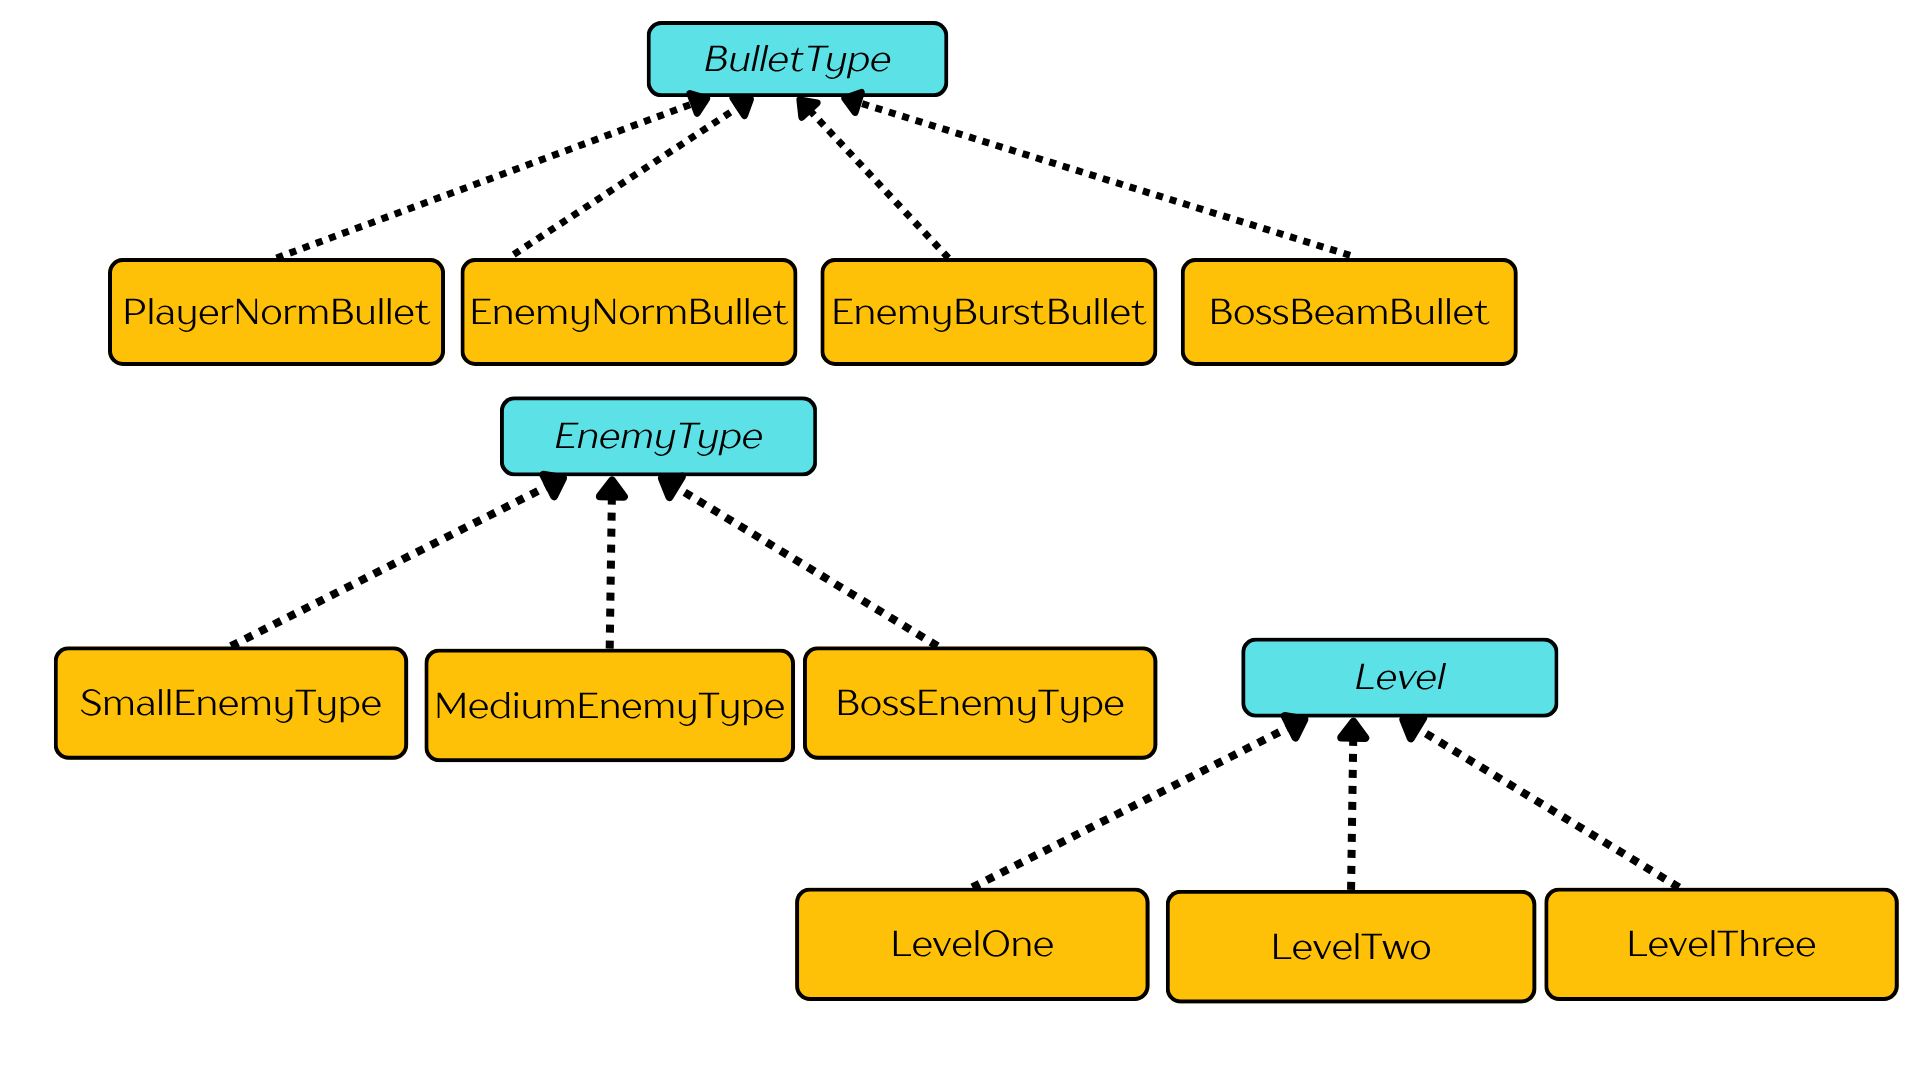
\includegraphics[width=0.95\textwidth]{misc/fig1_inheritance.png}
    \caption{Three inheritance hierarchies (BulletType, EnemyType, Level).
             Arrows point from child to parent (\emph{``inherits from''}).
             Shaded boxes are abstract bases; plain boxes are concrete subclasses.}
    \label{fig:inherit}
\end{figure}

\begin{figure}[H]
    \centering
    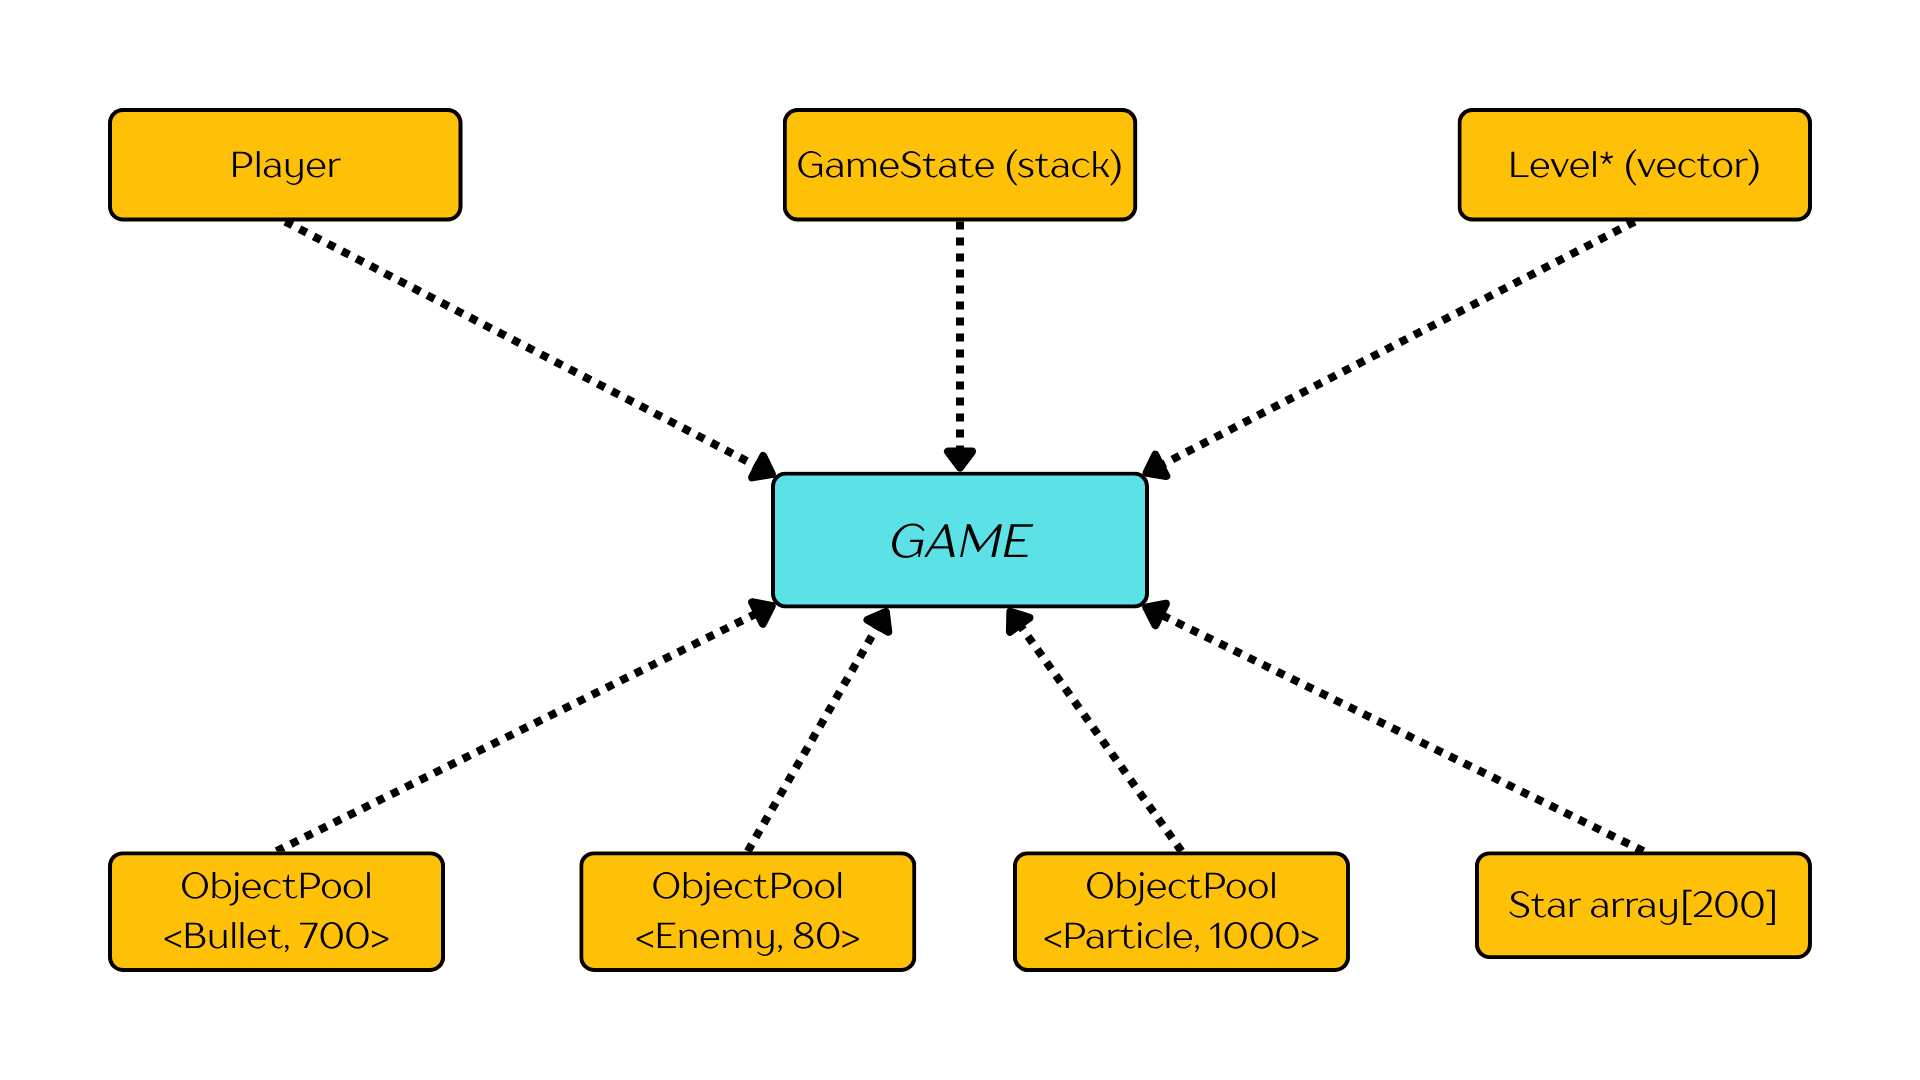
\includegraphics[width=0.80\textwidth]{misc/fig2_composition.png}
    \caption{Composition: the \texttt{Game} class \emph{owns} (has-a) all subsystems.
             Arrows labelled \texttt{has-a} mean ``contains as a member variable''.}
    \label{fig:compose}
\end{figure}

\subsection{Class and Struct Descriptions}

\subsubsection{Classes (with behaviour)}

\begin{table}[htbp]
    \centering
    \caption{Classes and their responsibilities}
    \label{tab:classes}
    \renewcommand{\arraystretch}{1.2}
    \small
    \begin{tabular}{|l|p{3.2cm}|p{5.8cm}|}
        \hline
        \textbf{Class} & \textbf{Responsibility} & \textbf{Key members} \\
        \hline
        \texttt{BulletType} & Identifies a bullet's category and owner & \texttt{id}, \texttt{playerBullet}, \texttt{getId()}, \texttt{isPlayerBullet()}, static singletons \texttt{PlayerNorm}, \texttt{EnemyNorm}, \texttt{EnemyBurst}, \texttt{BossBeam} \\
        \hline
        \texttt{PlayerNormBullet} & Player's straight-up shot & Inherits BulletType with id=0, playerBullet=true \\
        \hline
        \texttt{EnemyNormBullet} & Basic aimed enemy shot & id=3, playerBullet=false \\
        \hline
        \texttt{EnemyBurstBullet} & Spread-fire enemy shot & id=4, playerBullet=false \\
        \hline
        \texttt{BossBeamBullet} & Boss beam projectile & id=5, playerBullet=false \\
        \hline
        \texttt{BulletTypeRegistry} & Owns and initialises all four bullet-type singletons & Private members: one instance of each concrete subclass; constructor wires static pointers; destructor clears them to \texttt{nullptr}; copy disabled (\texttt{= delete}) \\
        \hline
        \texttt{EnemyType} & Stores the stat profile for one enemy category & \texttt{maxHp}, \texttt{shootInterval}, \texttt{scoreValue}, \texttt{moveSpeed}, \texttt{radius}, \texttt{kind}; static singletons \texttt{Small}, \texttt{Medium}, \texttt{Boss} \\
        \hline
        \texttt{SmallEnemyType} & Fast, weak enemy & 30\,HP, interval 2.2s, radius 16px, worth 50 pts \\
        \hline
        \texttt{MediumEnemyType} & Tanky spread-shooter & 80\,HP, interval 1.8s, radius 22px, worth 120 pts \\
        \hline
        \texttt{BossEnemyType} & End-of-level boss & 1200\,HP, interval 0.8s, radius 60px, worth 2000 pts \\
        \hline
        \texttt{EnemyTypeRegistry} & Owns and initialises all three enemy-type singletons & Same RAII pattern as \texttt{BulletTypeRegistry}; constructor assigns \texttt{Small}, \texttt{Medium}, \texttt{Boss} pointers; destructor sets them to \texttt{nullptr}; copy disabled \\
        \hline
        \texttt{GameState} & Tracks which screen is active & \texttt{id}; \texttt{operator==}, \texttt{operator!=}; static constants \texttt{Home}, \texttt{LevelSelect}, \texttt{Playing}, \texttt{Paused}, \texttt{GameOver}, \texttt{LevelComplete} \\
        \hline
        \texttt{Player} & Encapsulates all player state and behaviour & pos, hp, maxHp, speed, lives, score, timers; movement, clamping, damage, healing, score accumulation \\
        \hline
        \texttt{Level} & Abstract base for a playable level & name, desc, events (SpawnEvent list), planetTexture; pure virtual \texttt{buildWaves()}, \texttt{getDuration()}, \texttt{getPlanetTexturePath()} \\
        \hline
        \texttt{LevelOne/Two/Three} & Concrete level implementations & Override \texttt{buildWaves()} with a timed enemy schedule \\
        \hline
        \texttt{ObjectPool<T,N>} & Fixed-size object recycler & \texttt{items[N]}; \texttt{alloc()}, \texttt{clearAll()}, \texttt{countActive()} \\
        \hline
        \texttt{Game} & Central orchestrator & Owns all subsystems; implements init, run, update, collision, spawning; includes \texttt{sf::Music} for background audio; rendering split into \texttt{Game\_graphics.cpp} \\
        \hline
    \end{tabular}
\end{table}

\subsubsection{Data Structs (plain data containers)}

\begin{table}[H]
    \centering
    \caption{Data structs used as game objects}
    \label{tab:structs}
    \renewcommand{\arraystretch}{1.4}
    \begin{tabular}{|l|p{4.2cm}|p{5.5cm}|}
        \hline
        \textbf{Struct} & \textbf{Represents} & \textbf{Key fields} \\
        \hline
        \texttt{Bullet} & One active projectile & pos, vel, dmg, \texttt{BulletType*} type, on \\
        \hline
        \texttt{Enemy} & One active enemy & pos, vel, hp, maxHp, \texttt{EnemyType*} type, shootTimer, shootInterval, path, pathIndex, angle, pulse, scoreValue, moveSpeed, on \\
        \hline
        \texttt{Particle} & One explosion spark & pos, vel, colorStart, colorEnd, life, maxLife, size, on \\
        \hline
        \texttt{SpawnEvent} & A scheduled group spawn & time, etype, startPos, path, count, xSpacing, delay, fired \\
        \hline
        \texttt{SpawnJob} & One pending individual spawn & etype, startPos, delayRemaining, path, hp, maxHp, shootInterval, scoreValue, moveSpeed \\
        \hline
        \texttt{Star} & One background star & pos, speed, brightness, size \\
        \hline
    \end{tabular}
\end{table}

\begin{notebox}
\textbf{Why separate Struct from Class?}
A \emph{struct} in this project is a passive data container --- it holds values
but has no methods other than a default constructor.
A \emph{class} has active behaviour: it enforces invariants, provides
getters/setters, and contains logic. This distinction keeps data simple and
behaviour organised.
\end{notebox}

\subsection{OOP Concepts Summary}

\begin{table}[H]
    \centering
    \caption{OOP concepts used and where they appear}
    \label{tab:oop}
    \renewcommand{\arraystretch}{1.4}
    \begin{tabular}{|l|p{9cm}|}
        \hline
        \textbf{OOP Concept} & \textbf{Where and how it is used} \\
        \hline
        Encapsulation & \texttt{Player} class: all fields are \texttt{private}; external code uses getters and setters only \\
        \hline
        Inheritance & Three hierarchies: BulletType, EnemyType, Level (each abstract base + concrete subclasses) \\
        \hline
        Polymorphism & \texttt{Level::buildWaves()}, \texttt{getDuration()}, and \texttt{getPlanetTexturePath()} are pure virtual; \texttt{Game} calls them without knowing the concrete type \\
        \hline
        Abstract Classes & \texttt{BulletType}, \texttt{EnemyType}, and \texttt{Level} cannot be instantiated directly because they have pure virtual destructors or methods \\
        \hline
        Templates & \texttt{ObjectPool<T,N>} works for \texttt{Bullet}, \texttt{Enemy}, and \texttt{Particle} using the same code \\
        \hline
        Operator Overloading & \texttt{Player::operator+=(int)} adds score; \texttt{GameState::operator==} and \texttt{operator!=} compare states \\
        \hline
        Static Members & \texttt{BulletType::PlayerNorm}, \texttt{EnemyType::Small}, \texttt{GameState::Home} etc. --- global singletons accessed through the class name \\
        \hline
        Exception Handling & \texttt{AssetLoadException} and \texttt{InvalidLevelException} (custom classes inheriting \texttt{std::runtime\_error}) \\
        \hline
        Virtual Destructor & All abstract base classes (\texttt{BulletType}, \texttt{EnemyType}, \texttt{Level}) declare \texttt{virtual \textasciitilde{}Base()} so derived objects are safely deleted via a base pointer \\
        \hline
        Composition (has-a) & \texttt{Game} contains \texttt{Player}, three \texttt{ObjectPool} instances, a \texttt{vector<Level*>}, and a \texttt{stack<GameState>} as member variables \\
        \hline
        Recursion & \texttt{Game::spawnExplosion()} calls itself with a smaller particle count and reduced depth to create layered explosion effects \\
        \hline
    \end{tabular}
\end{table}

% ─────────────────────────────────────────────────────────────────────────
\section{Implementation}
% ─────────────────────────────────────────────────────────────────────────

\subsection{Development Environment}
\begin{itemize}
    \item \textbf{Language:} C++17
    \item \textbf{Graphics \& Audio library:} SFML 2.x (Simple and Fast Multimedia Library) --- graphics, window, and audio modules
    \item \textbf{Build system:} CMake with \texttt{CMakePresets.json}
    \item \textbf{IDE:} Visual Studio Code
    \item \textbf{Version control:} Git / GitHub (\texttt{hamza-branch})
    \item \textbf{Platform:} Windows 11
\end{itemize}

% ─────────────────────────────────────────────────────────────────────────
\subsection{Encapsulation --- The Player Class}

\begin{conceptbox}{Encapsulation}
Encapsulation means bundling data and the methods that operate on it inside
a single class, and hiding the internal details from the rest of the program.
Think of it like a vending machine: you press a button (the public interface),
and the internal mechanics (the private data) do the work --- you never reach
inside to grab the product yourself.
\end{conceptbox}

The \texttt{Player} class is the clearest example of encapsulation in the
project. Every field --- position, HP, lives, timers --- is declared
\texttt{private}. External code (including \texttt{Game}) can only interact
with the player through a controlled public interface.

\begin{lstlisting}[caption={Player class skeleton (Player.h)}]
class Player {
private:
    // position, hp, maxHp, speed, lives, score
    // shootTimer, iframeTimer, shieldTimer, tilt, alive

public:
    // Getters: getPos(), getHp(), getLives(), getScore(), isAlive(), ...
    void takeDamage(float d);       // reduces hp
    void heal(float h);             // increases hp, capped at maxHp
    void loseLife();                // decrements lives
    void clampToArena();            // keeps ship inside the play area
    Player& operator+=(int bonus);  // adds score (operator overload)
};
\end{lstlisting}

\textbf{Why this matters:} If \texttt{hp} were \texttt{public}, any code
could write \texttt{player.hp = -999} by accident. The \texttt{private}
keyword makes that a compile error --- only \texttt{takeDamage()} and
\texttt{heal()} can change health, and they do so safely.

% ─────────────────────────────────────────────────────────────────────────
\subsection{Inheritance --- Three Class Hierarchies}

\begin{conceptbox}{Inheritance}
Inheritance lets one class (the \emph{child} or \emph{derived} class) reuse
the code of another class (the \emph{parent} or \emph{base} class) and then
add or change specific behaviour. Think of it as a template: a ``Vehicle'' base
class defines that all vehicles have a speed and can move; a ``Car'' child
inherits those properties and adds four wheels; a ``Boat'' child adds a hull.
\end{conceptbox}

\subsubsection{Bullet Type Hierarchy}

We need to distinguish four kinds of bullets at runtime without comparing
raw integers everywhere. Each bullet type is a class:

\begin{lstlisting}[caption={BulletType hierarchy skeleton (BulletType.h)}]
class BulletType {          // abstract base -- defines the interface
    int id; bool playerBullet;
public:
    virtual ~BulletType() {}
    int getId() const; bool isPlayerBullet() const;
    static BulletType *PlayerNorm, *EnemyNorm, *EnemyBurst, *BossBeam;
};
// Concrete subclasses -- each hard-codes its own id
class PlayerNormBullet : public BulletType { /* id=0, player bullet */ };
class EnemyNormBullet  : public BulletType { /* id=3, enemy bullet  */ };
class EnemyBurstBullet : public BulletType { /* id=4, burst bullet  */ };
class BossBeamBullet   : public BulletType { /* id=5, boss beam     */ };
\end{lstlisting}

The four concrete objects are owned and managed by a \texttt{BulletTypeRegistry}
class defined at the bottom of \texttt{BulletType.h}. The static pointer
declarations and registry activations have been consolidated into
\texttt{main.cpp}, where the registries are created as local variables at the
top of \texttt{main()} --- \emph{before} the \texttt{Game} object --- ensuring
the singletons are valid for the entire programme lifetime:

\begin{lstlisting}[caption={BulletTypeRegistry --- RAII singleton manager (BulletType.h)}]
class BulletTypeRegistry {
private:
    PlayerNormBullet playerNorm;   // owned by value -- no heap allocation
    EnemyNormBullet  enemyNorm;
    EnemyBurstBullet enemyBurst;
    BossBeamBullet   bossBeam;
public:
    BulletTypeRegistry() {
        BulletType::PlayerNorm  = &playerNorm;   // wire static pointers
        BulletType::EnemyNorm   = &enemyNorm;
        BulletType::EnemyBurst  = &enemyBurst;
        BulletType::BossBeam    = &bossBeam;
    }
    ~BulletTypeRegistry() {
        BulletType::PlayerNorm = nullptr;        // safe teardown at exit
        BulletType::EnemyNorm  = nullptr;
        BulletType::EnemyBurst = nullptr;
        BulletType::BossBeam   = nullptr;
    }
    BulletTypeRegistry(const BulletTypeRegistry&)            = delete;
    BulletTypeRegistry& operator=(const BulletTypeRegistry&) = delete;
};
\end{lstlisting}

\begin{lstlisting}[caption={All static definitions and registry activation consolidated in main.cpp}]
// Static pointer definitions (must appear in exactly one .cpp file)
BulletType *BulletType::PlayerNorm = nullptr;
BulletType *BulletType::EnemyNorm  = nullptr;
BulletType *BulletType::EnemyBurst = nullptr;
BulletType *BulletType::BossBeam   = nullptr;

EnemyType *EnemyType::Small  = nullptr;
EnemyType *EnemyType::Medium = nullptr;
EnemyType *EnemyType::Boss   = nullptr;

const GameState GameState::Home(0);
// ... other GameState constants ...

int main() {
    BulletTypeRegistry registryBullet;  // constructor wires BulletType statics
    EnemyTypeRegistry  registry;         // constructor wires EnemyType statics
    try {
        Game game;
        game.init();
        game.run();
    } catch (...) { ... }
    // registries destroyed here -- destructors clear statics to nullptr
}
\end{lstlisting}

\textbf{Why not just use integers?} Using class pointers means the compiler
checks types. Comparing \texttt{b.type == BulletType::PlayerNorm} is
self-documenting and safe. Using \texttt{b.type == 0} would compile
even if you accidentally wrote \texttt{b.type == 100}.

\textbf{Why consolidate into main.cpp?} C++ requires that each static member
variable be \emph{defined} in exactly one translation unit. Placing all
definitions in one file (\texttt{main.cpp}) makes the ownership explicit and
eliminates three separate \texttt{.cpp} files (\texttt{BulletType.cpp},
\texttt{EnemyType.cpp}, \texttt{GameState.cpp}), simplifying the build.
The registry local variables in \texttt{main()} follow the RAII principle:
they are constructed before the game starts and destroyed after it ends,
with full lifecycle control and no hidden global state.

\subsubsection{Enemy Type Hierarchy}

Enemy types follow the same pattern but carry meaningful gameplay data:

\begin{lstlisting}[caption={EnemyType hierarchy skeleton (EnemyType.h)}]
class EnemyType {       // abstract base -- stores gameplay stats
    // maxHp, shootInterval, scoreValue, moveSpeed, radius, kind
public:
    virtual ~EnemyType() {}
    // Getters: getMaxHp(), getShootInterval(), getScoreValue(), ...
    static EnemyType *Small, *Medium, *Boss;
};
// Stats baked in: (hp, shootInterval, score, speed, radius, kind)
class SmallEnemyType  : public EnemyType { /* 30 HP,   2.2s, 50 pts  */ };
class MediumEnemyType : public EnemyType { /* 80 HP,   1.8s, 120 pts */ };
class BossEnemyType   : public EnemyType { /* 1200 HP, 0.8s, 2000 pts */ };
\end{lstlisting}

\textbf{Singleton management:} \texttt{EnemyType.h} also defines an
\texttt{EnemyTypeRegistry} class that owns the three concrete instances and wires
the static pointers in its constructor, following the same RAII pattern as
\texttt{BulletTypeRegistry}. One \texttt{static EnemyTypeRegistry registry}
in \texttt{EnemyType.cpp} activates everything at programme start and performs
safe teardown at exit.

\subsubsection{Level Hierarchy}

The \texttt{Level} base class defines the \emph{interface} that every level
must satisfy. The concrete subclasses fill in the details:

\begin{lstlisting}[caption={Level abstract base class skeleton (Level.h)}]
class Level {           // abstract base
protected:
    // name, desc, events (wave schedule), planetTexture

public:
    virtual ~Level() {}
    // Pure virtual -- every subclass MUST implement:
    virtual float       getDuration()          const = 0;
    virtual std::string getPlanetTexturePath() const = 0;
    virtual void        buildWaves()                 = 0;
    virtual void renderPlanet(sf::RenderWindow& w);  // has default impl.
};
class LevelOne   : public Level { /* 55s, planet1.png */ };
class LevelTwo   : public Level { /* 65s, planet2.png */ };
class LevelThree : public Level { /* 80s, planet3.png, two bosses */ };
\end{lstlisting}

% ─────────────────────────────────────────────────────────────────────────
\subsection{Polymorphism --- Same Call, Different Behaviour}

\begin{conceptbox}{Polymorphism}
Polymorphism means ``many forms.'' When you have a pointer to a base class,
calling a \texttt{virtual} function on it will automatically invoke the
\emph{correct overridden version} in the derived class --- even though the
pointer only ``knows'' about the base. The decision happens at runtime, not
at compile time. This is called \emph{dynamic dispatch}.
\end{conceptbox}

In \texttt{Game.cpp}, the game stores levels as base-class pointers and
calls the virtual functions without needing to know which level is loaded:

\begin{lstlisting}[caption={Polymorphic level calls in Game.cpp}]
std::vector<Level *> levels;   // stores LevelOne*, LevelTwo*, or LevelThree*

// During initialisation -- all three calls go through the base pointer:
for (int i = 0; i < levels.size(); i++) {
    levels[i]->buildWaves();   // calls LevelOne::buildWaves() OR
                               // LevelTwo::buildWaves() OR LevelThree::buildWaves()
    levels[i]->loadPlanet();   // calls Level::loadPlanet() (base version)
}

// During gameplay rendering:
void Game::renderBackground() {
    levels[currentLevel]->renderPlanet(window);  // correct planet drawn automatically
}
\end{lstlisting}

\textbf{The key insight:} \texttt{Game} never writes \texttt{if (level == 1) do X; else if (level == 2) do Y}. The virtual function dispatch table handles the routing. Adding a fourth level in the future requires zero changes to \texttt{Game.cpp}.

% ─────────────────────────────────────────────────────────────────────────
\subsection{Templates --- The ObjectPool}

\begin{conceptbox}{Templates}
A template is a class or function that is parameterised by a type. You write
the logic once and the compiler generates a separate, correctly-typed version
for each type you use it with. It is like a cookie cutter: the cutter (the
template) is the same; the dough (the type) changes.
\end{conceptbox}

The game needs to manage up to 700 bullets, 80 enemies, and 1000 particles
efficiently. Allocating and freeing individual objects every frame would be
slow and could cause memory fragmentation. Instead, we use a fixed-size
\emph{object pool}: a statically-allocated array where ``free'' objects are
recycled rather than deleted.

\begin{lstlisting}[caption={ObjectPool template class (GameData.h)}]
template <class T, int N>
class ObjectPool
{
private:
    std::array<T, N> items;   // fixed array -- allocated once, never reallocated

public:
    ObjectPool() {
        for (int i = 0; i < N; i++)
            items[i].on = false;   // all slots start as "free"
    }

    int  capacity()  const { return N; }
    T&   at(int i)         { return items[i]; }
    const T& at(int i) const { return items[i]; }

    // Find the first free slot and return a pointer to it
    T* alloc() {
        for (int i = 0; i < N; i++) {
            if (!items[i].on)
                return &items[i];
        }
        return nullptr;   // pool is full -- caller must handle this
    }

    void clearAll() {
        for (int i = 0; i < N; i++)
            items[i].on = false;
    }

    int countActive() const {
        int c = 0;
        for (int i = 0; i < N; i++) if (items[i].on) c++;
        return c;
    }
};
\end{lstlisting}

The three instantiations in the \texttt{Game} class:

\begin{lstlisting}[caption={Three pool instances in Game.h}]
ObjectPool<Bullet,   MAX_BULLETS>   bullets;    // 700 slots
ObjectPool<Enemy,    MAX_ENEMIES>   enemies;    //  80 slots
ObjectPool<Particle, MAX_PARTICLES> particles;  // 1000 slots
\end{lstlisting}

The template is written once; the compiler generates three separate, correctly-typed arrays. When a bullet is needed, \texttt{bullets.alloc()} finds a free slot and returns a pointer to it. When the bullet goes off-screen, \texttt{b.on = false} marks the slot as reusable --- no \texttt{new} or \texttt{delete} involved.

% ─────────────────────────────────────────────────────────────────────────
\subsection{Operator Overloading}

\begin{conceptbox}{Operator Overloading}
C++ lets you redefine what standard operators (\texttt{+}, \texttt{=},
\texttt{==}, etc.) mean for your custom class. This allows objects to be
used with familiar syntax rather than verbose method calls.
\end{conceptbox}

Two operator overloads appear in the project:

\subsubsection{Player::operator+= (score addition)}

\begin{lstlisting}[caption={Score addition via operator overload (Player.h)}]
// Instead of writing: player.addScore(e.scoreValue);
// We can write:       player += e.scoreValue;
Player& operator+=(int scoreBonus) {
    score += scoreBonus;
    return *this;
}
\end{lstlisting}

Used in \texttt{Game.cpp} when an enemy is destroyed:
\begin{lstlisting}[caption={Using the overloaded operator in Game.cpp}]
if (e.hp <= 0.f) {
    e.on = false;
    player += e.scoreValue;   // clean, readable syntax
}
\end{lstlisting}

\subsubsection{GameState::operator== and operator!=}

\begin{lstlisting}[caption={Comparison operators on GameState (GameState.h)}]
bool operator==(const GameState& o) const { return id == o.id; }
bool operator!=(const GameState& o) const { return id != o.id; }
\end{lstlisting}

Used throughout \texttt{Game.cpp} for readable state checks:
\begin{lstlisting}[caption={State comparison in Game.cpp}]
GameState current = stateStack.top();
if (current == GameState::Playing) { update(dt); }
\end{lstlisting}

% ─────────────────────────────────────────────────────────────────────────
\subsection{Exception Handling --- Custom Exception Classes}

\begin{conceptbox}{Exception Handling}
Exceptions are a mechanism for signalling that something went wrong without
cluttering normal code with error checks everywhere. You \texttt{throw} an
exception when an error occurs, and \texttt{catch} it at a higher level where
you know how to handle it. Custom exception classes (which inherit from
\texttt{std::exception}) let you distinguish different kinds of errors.
\end{conceptbox}

Two custom exceptions are defined inside \texttt{Game.cpp}:

\begin{lstlisting}[caption={Custom exception classes (Game.cpp)}]
// Thrown when a texture, font, or other asset cannot be loaded from disk
class AssetLoadException : public std::runtime_error {
public:
    AssetLoadException() : std::runtime_error("Failed to load asset") {}
};

// Thrown when startLevel() is called with an invalid index
class InvalidLevelException : public std::runtime_error {
public:
    InvalidLevelException() : std::runtime_error("Invalid level") {}
};
\end{lstlisting}

These are thrown and caught in \texttt{Game::init()} and
\texttt{Game::startLevel()}:

\begin{lstlisting}[caption={Throwing and catching exceptions (Game.cpp)}]
// In Game::init() -- missing assets are non-fatal; the game warns and continues
try {
    loadTextureOrThrow(shipTexture, "assets/textures/spaceship.png");
    loadTextureOrThrow(smallEnemyTexture, "assets/textures/alien1.png");
    // ... more assets ...
} catch (const AssetLoadException& ex) {
    std::cerr << "Asset warning: " << ex.what() << "\n";
}

// In Game::startLevel() -- an invalid index is a programming bug
void Game::startLevel(int index) {
    if (index < 0 || index >= (int)levels.size())
        throw InvalidLevelException();
    // ...
}

// In main.cpp -- the outermost safety net
int main() {
    try {
        Game game;
        game.init();
        game.run();
    } catch (const std::exception& ex) {
        std::cerr << "Fatal error: " << ex.what() << std::endl;
        return 1;
    }
}
\end{lstlisting}

% ─────────────────────────────────────────────────────────────────────────
\subsection{The Wave Spawn System}

Understanding how enemies appear on screen requires following a
three-stage pipeline. This section walks through it in plain language.

\subsubsection{Stage 1 --- SpawnEvent: the schedule}

When a level is loaded, \texttt{buildWaves()} fills a list of
\texttt{SpawnEvent} objects. Each one is a row in the level's timetable:

\begin{lstlisting}[caption={A single SpawnEvent (from LevelOne::buildWaves in Level.cpp)}]
// At t = 14.0 seconds, spawn 4 Small enemies starting at x=240,
// following the "sweep centre" path, 50px apart, 0.25s between each.
events.push_back(makeEvent(
    14.0f,              // fire at t=14 seconds into the level
    EnemyType::Small,   // what type of enemy
    sf::Vector2f(240, -40),  // group starting position (above screen)
    pathSweepCenter(),  // waypoints the group follows
    4,                  // 4 enemies in this group
    50.f,               // 50px horizontal spacing between them
    0.25f               // 0.25s delay between individual spawns
));
\end{lstlisting}

Nothing has spawned yet. This is just a schedule.

\subsubsection{Stage 2 --- checkSpawns(): firing events into the queue}

Every frame, the game increments a timer and checks whether any event's
scheduled time has passed:

\begin{lstlisting}[caption={Firing events from the schedule (Game.cpp)}]
void Game::checkSpawns(float dt) {
    std::vector<SpawnEvent>& evs = levels[currentLevel]->getEvents();
    for (int i = 0; i < evs.size(); i++) {
        SpawnEvent& ev = evs[i];
        if (!ev.fired && levelTimer >= ev.time) {
            ev.fired = true;
            for (int k = 0; k < ev.count; k++) {
                SpawnJob job;
                job.etype          = ev.etype;
                job.startPos.x    += (k - (ev.count-1)/2.f) * ev.xSpacing;
                job.delayRemaining = k * ev.delay;  // stagger each enemy
                job.path           = ev.path;
                spawnQueue.push(job);   // queued -- not yet alive
            }
        }
    }
}
\end{lstlisting}

The 4-enemy event above would push 4 SpawnJobs with delays of
0s, 0.25s, 0.5s, and 0.75s respectively.

\subsubsection{Stage 3 --- Draining the queue into live enemies}

Each frame, the front of the queue is checked. When its delay reaches
zero, the enemy is activated in the pool:

\begin{lstlisting}[caption={Activating a queued enemy (Game.cpp)}]
while (!spawnQueue.empty()) {
    SpawnJob& front = spawnQueue.front();
    front.delayRemaining -= dt;
    if (front.delayRemaining <= 0.f) {
        spawnEnemyFromJob(front);   // writes into an ObjectPool slot
        spawnQueue.pop();
    } else {
        break;  // rest of queue is still waiting
    }
}

void Game::spawnEnemyFromJob(const SpawnJob& job) {
    Enemy* e = enemies.alloc();   // grab a free pool slot
    if (!e) return;
    e->on           = true;       // mark the slot as active
    e->type         = job.etype;
    e->pos          = job.startPos;
    e->hp           = job.hp;
    e->path         = job.path;
    e->pathIndex    = 0;
    e->shootTimer   = job.shootInterval * randFloat(0.3f, 1.0f);
}
\end{lstlisting}

\subsubsection{Enemy Movement along Waypoints}

Once alive, each enemy follows a list of 2D waypoints:

\begin{lstlisting}[caption={Waypoint movement (Game.cpp)}]
if (e.pathIndex < e.path.size()) {
    sf::Vector2f target   = e.path[e.pathIndex];
    sf::Vector2f toTarget = target - e.pos;
    float dist = vlen(toTarget);     // vector length from Utils.h
    if (dist < 8.f)
        e.pathIndex++;               // close enough -- advance to next waypoint
    else {
        sf::Vector2f dir = vnorm(toTarget);   // normalise direction
        e.pos += dir * e.moveSpeed * dt;      // move toward waypoint
    }
} else {
    e.pos.y += 100.f * dt;           // ran out of waypoints -- drift off-screen
    if (e.pos.y > 800.f) e.on = false;
}
\end{lstlisting}

% ─────────────────────────────────────────────────────────────────────────
\subsection{Recursion --- Layered Explosion System}

\begin{conceptbox}{Recursion}
Recursion is when a function calls itself with a smaller version of the
same problem, until it reaches a base case and stops. It is useful whenever
a task can be broken down into identical subtasks --- such as spawning
an explosion that itself spawns smaller explosions.
\end{conceptbox}

When an enemy is destroyed, \texttt{Game::spawnExplosion()} is called
recursively to produce layered, depth-based particle bursts. Each recursive
call spawns a smaller explosion at a nearby offset, creating a visually
rich chain effect:

\begin{lstlisting}[caption={Recursive explosion spawner (Game.cpp)}]
void Game::spawnExplosion(sf::Vector2f pos, sf::Color cStart,
                          sf::Color cEnd, int count, int depth) {
    // Base step: spawn particles at this position
    for (int i = 0; i < count; i++) {
        Particle* p = particles.alloc();
        if (!p) return;
        // ... set pos, vel, color, life
        p->on = true;
    }
    // Recursive step: spawn a smaller explosion nearby
    if (depth > 0) {
        float ox = randFloat(-20.f, 20.f);
        float oy = randFloat(-20.f, 20.f);
        spawnExplosion(pos + sf::Vector2f(ox, oy),
                       cStart, cEnd,
                       count / 2,   // fewer particles each time
                       depth - 1);  // base case: depth == 0
    }
}
\end{lstlisting}

\textbf{Base case:} \texttt{depth == 0} --- the function stops recursing.
\textbf{Recursive case:} each call spawns particles then calls itself
with \texttt{count/2} and \texttt{depth-1}. A depth-2 explosion produces
particles at 3 positions (1 + 1 + 1), each progressively smaller.

% ─────────────────────────────────────────────────────────────────────────
\subsection{Game Loop and State Machine}

The \texttt{GameState} class and a \texttt{std::stack} implement a simple
push/pop state machine. States are pushed onto the stack (e.g. Paused
on top of Playing) and popped to return to the previous screen.

\begin{figure}[H]
    \centering
    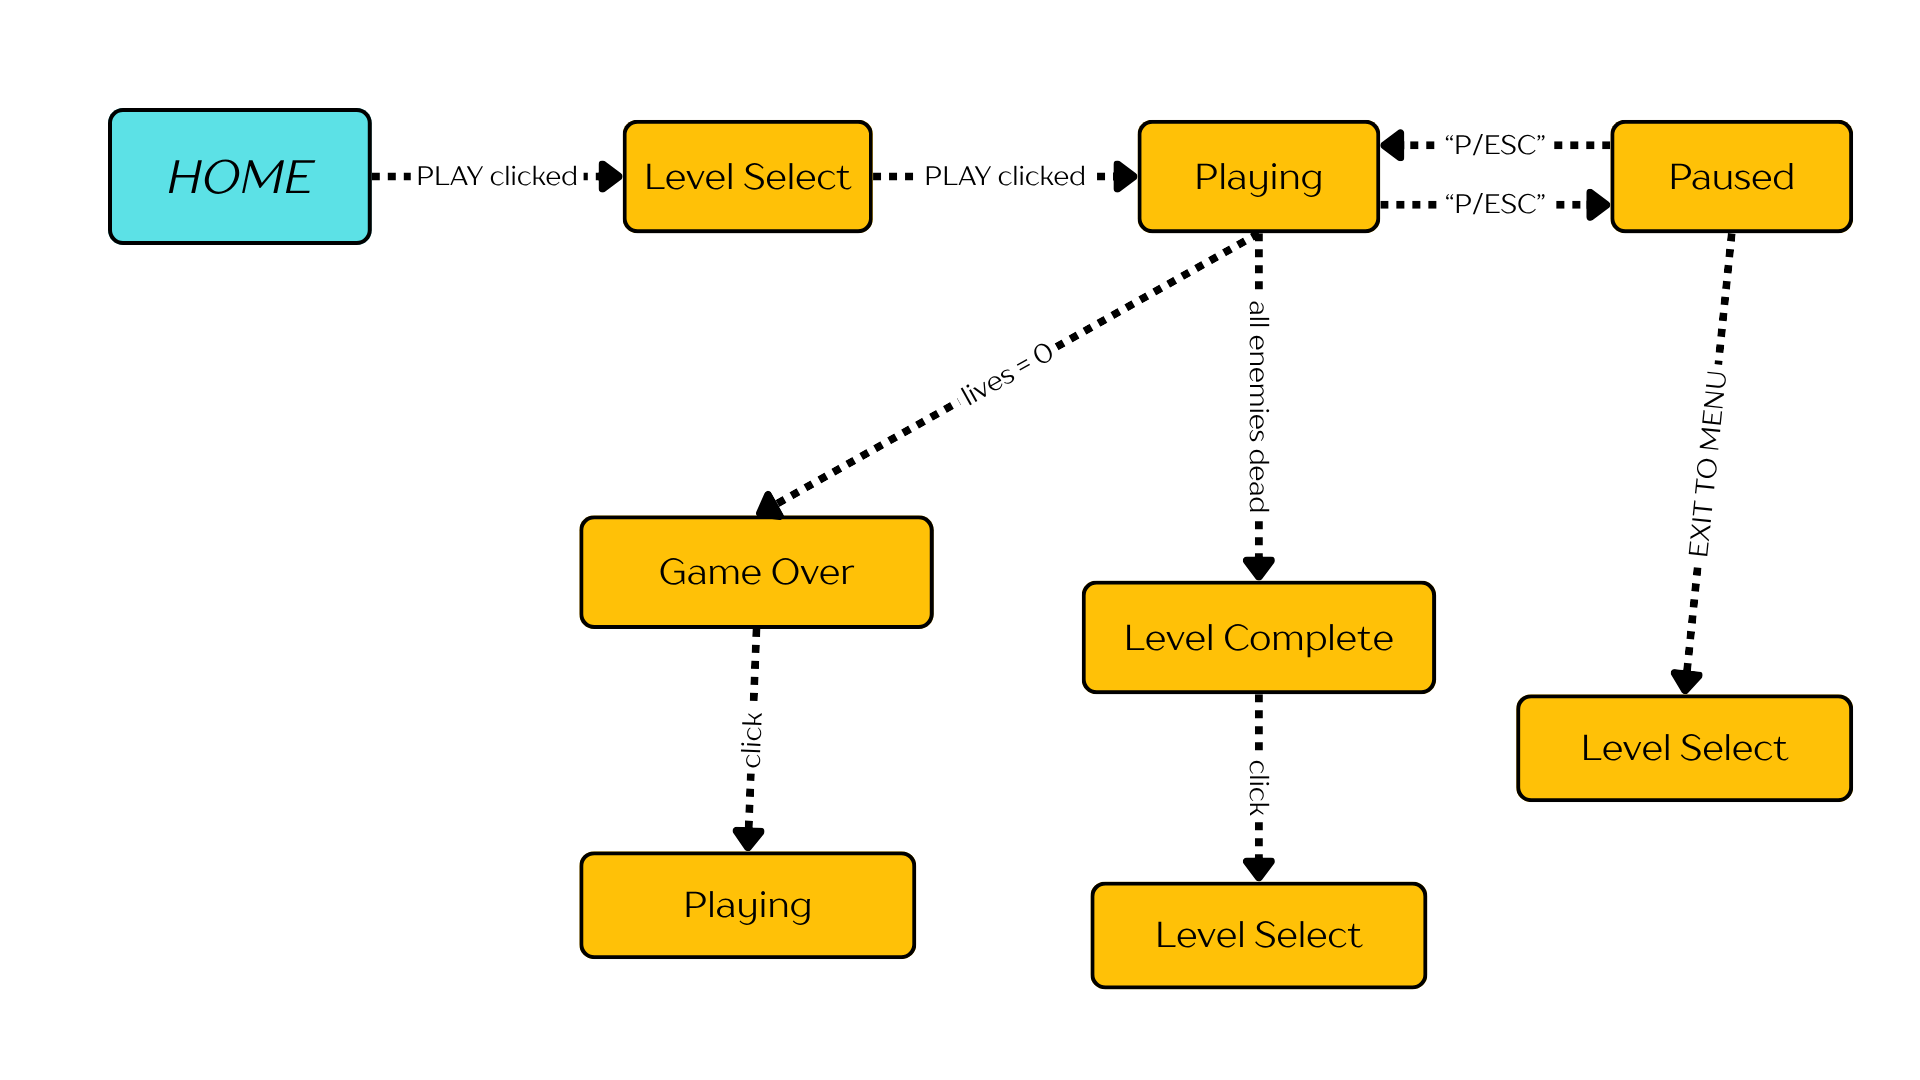
\includegraphics[width=0.85\textwidth]{misc/fig3_states.png}
    \caption{Game state transitions. Arrows show what action triggers each transition.}
    \label{fig:states}
\end{figure}

% ─────────────────────────────────────────────────────────────────────────
\section{Testing}
% ─────────────────────────────────────────────────────────────────────────

\subsection{Test Cases}

\begin{table}[H]
    \centering
    \caption{Edge Case and Exception Test Cases}
    \label{tab:tests}
    \renewcommand{\arraystretch}{1.3}
    \begin{tabular}{|c|p{3.8cm}|p{3.8cm}|c|}
        \hline
        \textbf{TC} & \textbf{Scenario} & \textbf{Expected Outcome} & \textbf{Pass?} \\
        \hline
        TC-01 & Hold Space to fire \textasciitilde700 bullets & Pool fills up; \texttt{alloc()} returns \texttt{nullptr}; no crash or out-of-bounds & \checkmark \\
        \hline
        TC-02 & Take damage immediately after a previous hit (iframes active) & Damage ignored for iframe duration; HP unchanged & \checkmark \\
        \hline
        TC-03 & Rename or delete a texture file; launch game & \texttt{AssetLoadException} caught; warning printed; game continues & \checkmark \\
        \hline
        TC-04 & Call \texttt{startLevel(-1)} programmatically & \texttt{InvalidLevelException} thrown and caught at outermost level in \texttt{main()} & \checkmark \\
        \hline
        TC-05 & Kill all enemies including boss & \texttt{isLevelClear()} returns true; Level Complete overlay shown & \checkmark \\
        \hline
    \end{tabular}
\end{table}

\subsection{Memory Leak Testing}

An earlier version of the code used \texttt{new} to create the
\texttt{BulletType} and \texttt{EnemyType} singletons, causing pointer leaks
because \texttt{delete} was never called. The fix introduced dedicated
\texttt{BulletTypeRegistry} and \texttt{EnemyTypeRegistry} classes. Each
registry owns its concrete instances as plain member variables (no heap
allocation), wires the static pointers in its constructor, and clears them to
\texttt{nullptr} in its destructor. The registry objects are now created as
local variables at the top of \texttt{main()}, giving them explicit lifetime
control: they are alive for the entire duration of the programme and
automatically cleaned up when \texttt{main()} returns.
All static member definitions were also consolidated into \texttt{main.cpp},
removing the need for the separate \texttt{BulletType.cpp},
\texttt{EnemyType.cpp}, and \texttt{GameState.cpp} files entirely.

% ─────────────────────────────────────────────────────────────────────────
\section{Expected Output --- Screenshots}
% ─────────────────────────────────────────────────────────────────────────

The following screenshots were captured from the running game. Each
illustrates a distinct screen or game state.

\begin{figure}[H]
    \centering
    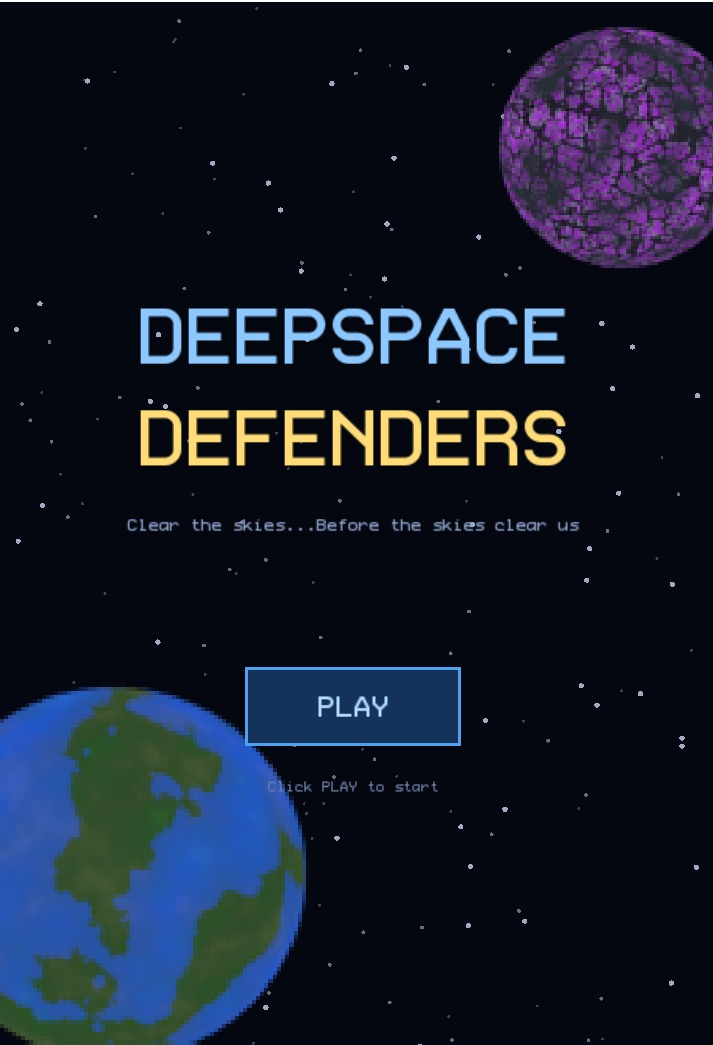
\includegraphics[width=0.75\textwidth]{misc/ss1_home.png}
    \caption{Home screen: title text, scrolling star background, two decorative
             planets, and the PLAY button.}
    \label{fig:ss_home}
\end{figure}

\begin{figure}[H]
    \centering
    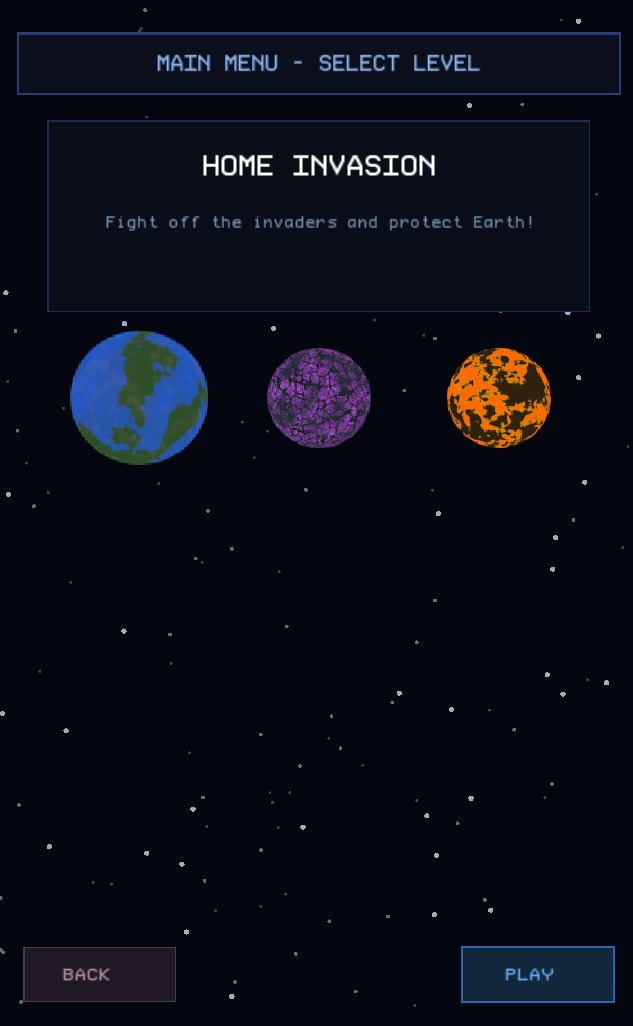
\includegraphics[width=0.75\textwidth]{misc/ss2_levelselect.png}
    \caption{Level Select screen: three planet buttons (the selected one is
             larger), level name and description preview, BACK and PLAY buttons.}
    \label{fig:ss_levelsel}
\end{figure}

\begin{figure}[H]
    \centering
    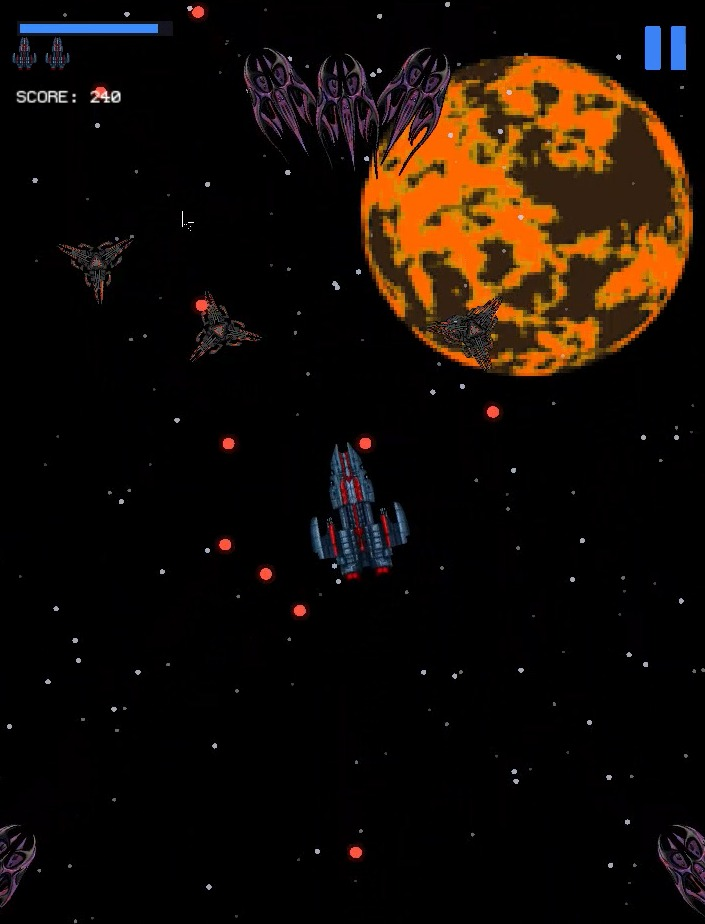
\includegraphics[width=0.75\textwidth]{misc/ss3_gameplay.png}
    \caption{Mid-game: player ship, enemy formation following waypoints,
             player bullets, HUD showing HP bar, lives, and score.}
    \label{fig:ss_play}
\end{figure}

\begin{figure}[H]
    \centering
    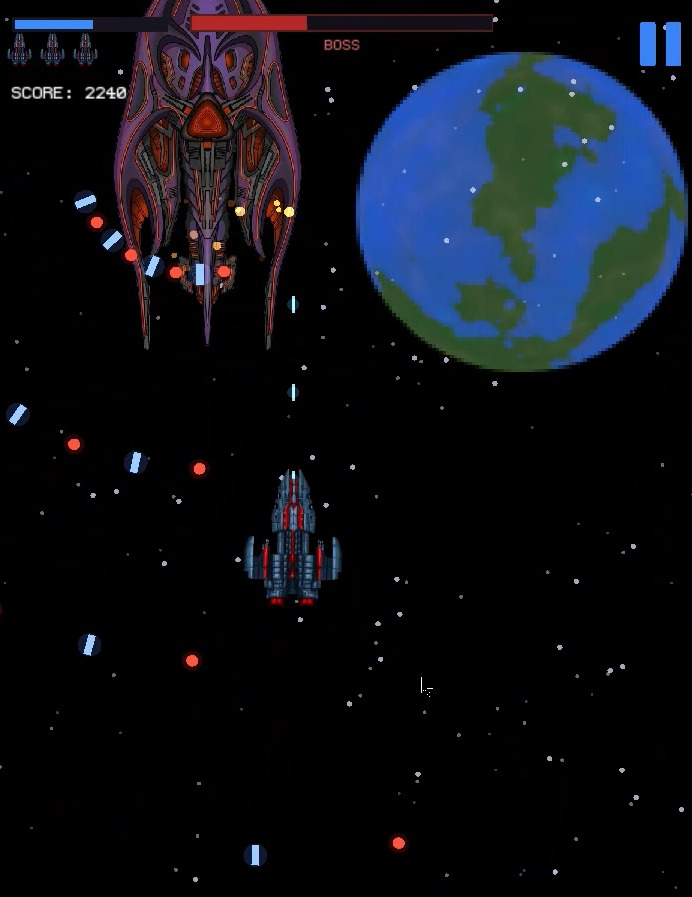
\includegraphics[width=0.75\textwidth]{misc/ss4_boss.png}
    \caption{Boss encounter: large boss sprite on screen, red boss HP bar
             centred at the top, particle explosions visible.}
    \label{fig:ss_boss}
\end{figure}

\begin{figure}[H]
    \centering
    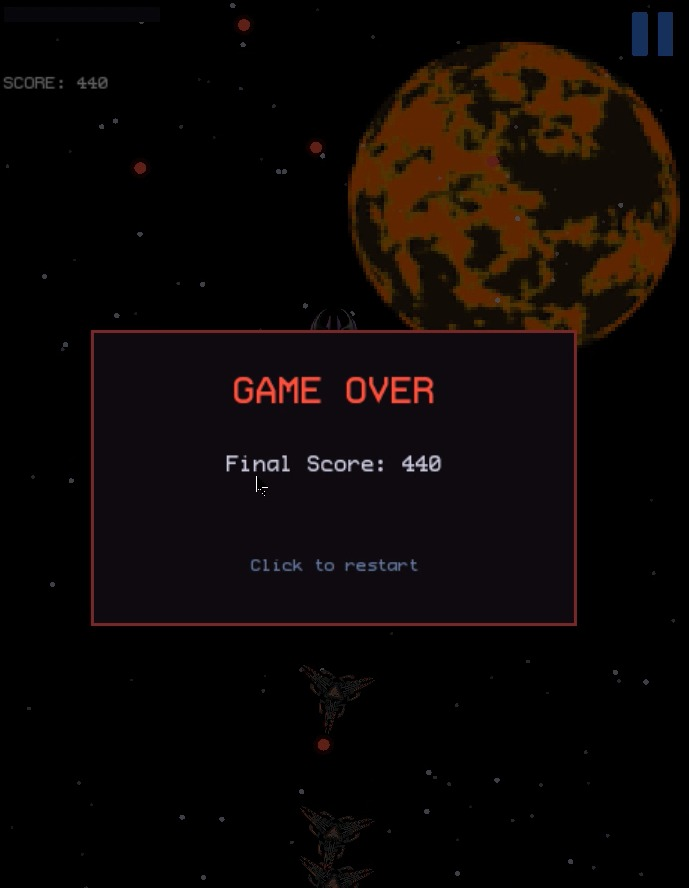
\includegraphics[width=0.75\textwidth]{misc/ss5_gameover.png}
    \caption{Game Over overlay: dimmed background, ``GAME OVER'' heading,
             final score, and ``Click to restart'' prompt.}
    \label{fig:ss_over}
\end{figure}

\begin{figure}[H]
    \centering
    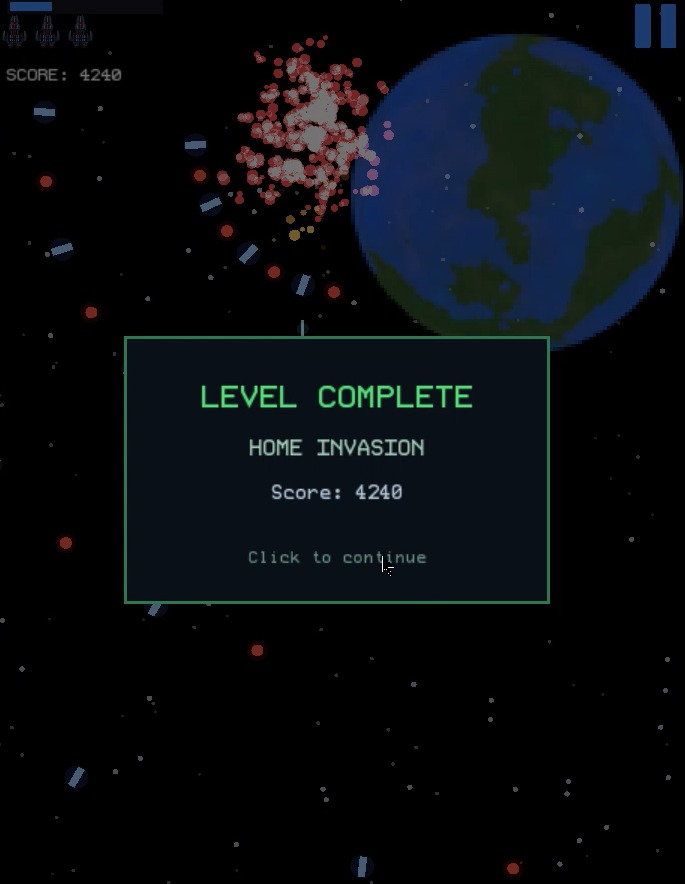
\includegraphics[width=0.75\textwidth]{misc/ss6_levelcomplete.png}
    \caption{Level Complete overlay: green panel with level name, score,
             and ``Click to continue'' prompt.}
    \label{fig:ss_done}
\end{figure}

% ─────────────────────────────────────────────────────────────────────────
\section{Results and Discussion}
% ─────────────────────────────────────────────────────────────────────────

\subsection{Results}

\begin{itemize}
    \item The game runs smoothly at 60 frames per second on standard hardware.
    \item All three levels are completable: Level One (55s), Level Two (65s),
          Level Three (80s, two bosses).
    \item Background music plays via \texttt{sf::Music} using OGG audio streaming.
    \item The \texttt{ObjectPool} successfully prevents runtime allocation:
          no \texttt{new} or \texttt{delete} occurs during gameplay.
    \item The three inheritance hierarchies (bullets, enemies, levels) are
          genuinely polymorphic --- \texttt{Game.cpp} never queries concrete
          types to decide which base-class method to call.
    \item The state machine handles all screen transitions cleanly, including
          nested states (Paused inside Playing).
    \item Rendering logic is fully separated into \texttt{Game\_graphics.cpp},
          keeping \texttt{Game.cpp} focused on game logic only.
\end{itemize}

\subsection{Analysis}

\begin{itemize}
    \item \textbf{ObjectPool vs dynamic allocation:} Checking 700 slots
          linearly to find a free bullet takes at most $700 \times 1$ comparisons
          per allocation. At 60 fps, with approximately 10 allocations per
          second, this is negligible. The benefit --- zero fragmentation,
          cache-friendly memory layout --- outweighs the linear scan.

    \item \textbf{Polymorphism overhead:} Virtual function calls add one
          pointer dereference per call (the vtable lookup). For the small
          number of calls per frame (3 level methods, up to 80 enemy type
          lookups), this overhead is unmeasurable.

    \item \textbf{Template code size:} The compiler generates three separate
          versions of \texttt{ObjectPool}. For three small instantiations,
          the binary size increase is negligible.
\end{itemize}

% ─────────────────────────────────────────────────────────────────────────
\section{Challenges and Solutions}
% ─────────────────────────────────────────────────────────────────────────

\subsection{Pointer Leaks from Static Singletons}
\textbf{Problem:} The initial implementation used \texttt{new} to create
the \texttt{BulletType} and \texttt{EnemyType} singleton objects. Because
no \texttt{delete} was ever called, memory analysis tools reported leaks.\\[4pt]
\textbf{Solution:} Introduced \texttt{BulletTypeRegistry} and
\texttt{EnemyTypeRegistry} classes following the RAII pattern. Each registry
owns its concrete type instances as plain member variables (no heap allocation).
The constructor wires the static pointers; the destructor sets them to
\texttt{nullptr}. A single \texttt{static} registry instance at file scope in
each \texttt{.cpp} is all that is needed. The registry objects are now declared
as local variables at the top of \texttt{main()}, giving them explicit lifetime
control and eliminating the need for three separate \texttt{.cpp} files.
Copy construction and assignment are explicitly \texttt{= delete}d to prevent
accidental duplication of the registry.\\[4pt]
\textbf{Learning:} Encapsulate resource initialisation and cleanup inside a
class using RAII. Placing registries as locals in \texttt{main()} gives the
clearest possible lifetime: they are alive exactly as long as the programme
runs, with no hidden static initialisation order issues.

\subsection{Enemies All Spawning at the Same Position}
\textbf{Problem:} When a wave of 4 enemies was triggered, all 4 appeared
at exactly the same $(x, y)$ coordinate, stacking on top of each other.\\[4pt]
\textbf{Solution:} The \texttt{xSpacing} field in \texttt{SpawnEvent} and
the offset calculation in \texttt{checkSpawns} distribute the starting
$x$ position of each enemy by \texttt{(k - (count-1)/2.0) * xSpacing},
centring the group around the event's \texttt{startPos}.\\[4pt]
\textbf{Learning:} Centre-offset arithmetic (shifting by half the total
width) is a common pattern for distributing UI or game elements evenly.

\subsection{Frame-rate-dependent Movement}
\textbf{Problem:} Early versions moved objects by a fixed number of pixels
per frame. On a faster machine (120 fps), the game ran twice as fast.\\[4pt]
\textbf{Solution:} All movement and timers are multiplied by \texttt{dt}
(delta time in seconds). At 60 fps, \texttt{dt $\approx$ 0.0167s}; at
120 fps, \texttt{dt $\approx$ 0.0083s}. The product is the same distance
per second regardless of frame rate.\\[4pt]
\textbf{Learning:} Always express game speed in units per \emph{second},
never per \emph{frame}.

% ─────────────────────────────────────────────────────────────────────────
\section{Future Work}
% ─────────────────────────────────────────────────────────────────────────

\begin{itemize}
    \item \textbf{Power-ups:} A \texttt{PowerUp} base class with subclasses
          for shield, speed boost, and rapid fire --- following the same
          inheritance pattern as \texttt{BulletType}.
    \item \textbf{High score persistence:} Write the score to a \texttt{.txt}
          file after each game over and display the top 5 on the home screen.
    \item \textbf{Sound:} SFML's \texttt{sf::SoundBuffer} and \texttt{sf::Sound}
          for shoot, explosion, and level-complete audio.
    \item \textbf{More levels and enemy patterns:} The level system is
          designed for extension --- adding \texttt{LevelFour} requires only
          a new subclass of \texttt{Level}, with zero changes to \texttt{Game.cpp}.
    \item \textbf{Unit testing:} Use Google Test to verify \texttt{ObjectPool}
          allocation/deallocation, \texttt{Player} damage/healing invariants,
          and spawn-queue ordering.
\end{itemize}

% ─────────────────────────────────────────────────────────────────────────
\section{Conclusion}
% ─────────────────────────────────────────────────────────────────────────

\begin{infobox}
\textbf{Deepspace Defenders} demonstrates that a complete, interactive
application --- one with real-time graphics, multiple screens, and live
game objects --- can be cleanly designed using fundamental OOP principles.
\end{infobox}

The project successfully applied all required OOP concepts:

\begin{itemize}
    \item \textbf{Encapsulation} protected the player's state from external
          corruption through private fields and a controlled public interface.
    \item \textbf{Inheritance} allowed three independent type hierarchies
          (bullets, enemies, levels) to share common structure while differing
          in specific behaviour.
    \item \textbf{Polymorphism} let the game loop interact with any level or
          enemy type through base-class pointers, making the code open to
          extension without modification.
    \item \textbf{Templates} produced a single, reusable memory pool that
          works for all live game objects without repeating code.
    \item \textbf{Operator overloading} made score addition and state
          comparison readable and idiomatic.
    \item \textbf{Custom exceptions} separated error-handling logic cleanly
          from normal gameplay logic.
\end{itemize}

The most important takeaway is that OOP is not about using the concepts
because they are required --- it is about using them because they solve a
real problem. Every concept listed above was chosen because it made the
code shorter, safer, or easier to extend. That is the true goal of
Object-Oriented design.

% ─────────────────────────────────────────────────────────────────────────
\newpage
\section*{References}
\addcontentsline{toc}{section}{References}
% ─────────────────────────────────────────────────────────────────────────

\begin{enumerate}[label={[\arabic*]}]
    \item B. Stroustrup, \textit{The C++ Programming Language}, 4th ed. Addison-Wesley, 2013.
    \item S. Meyers, \textit{Effective Modern C++}. O'Reilly Media, 2014.
    \item \textit{SFML Documentation}. [Online]. Available: \url{https://www.sfml-dev.org/documentation/}. [Accessed: \today].
    \item \textit{cppreference.com --- C++ Reference}. [Online]. Available: \url{https://en.cppreference.com}. [Accessed: \today].
    \item \textit{Game Programming Patterns} by Robert Nystrom. [Online]. Available: \url{https://gameprogrammingpatterns.com}. [Accessed: \today].
\end{enumerate}

% ─────────────────────────────────────────────────────────────────────────
\newpage
\appendix
\section{Complete Source Code}
\label{sec:code}
% ─────────────────────────────────────────────────────────────────────────

\subsection{GameData.h}
\begin{lstlisting}[caption={GameData.h --- all data structs and ObjectPool template}]
#pragma once
#include <SFML/Graphics.hpp>
#include <array>
#include <vector>
#include "BulletType.h"
#include "EnemyType.h"

struct Bullet  { sf::Vector2f pos, vel; float dmg; BulletType* type; bool on; };
struct Enemy   { sf::Vector2f pos, vel; float hp, maxHp; EnemyType* type;
                 float shootTimer, shootInterval, angle, pulse, moveSpeed;
                 int scoreValue, pathIndex; std::vector<sf::Vector2f> path; bool on; };
struct Particle{ sf::Vector2f pos, vel; sf::Color colorStart, colorEnd;
                 float life, maxLife, size; bool on; };
struct SpawnEvent { float time, xSpacing, delay; EnemyType* etype;
                    sf::Vector2f startPos; std::vector<sf::Vector2f> path;
                    int count; bool fired; };
struct SpawnJob   { EnemyType* etype; sf::Vector2f startPos;
                    float delayRemaining, hp, maxHp, shootInterval, moveSpeed;
                    int scoreValue; std::vector<sf::Vector2f> path; };
struct Star    { sf::Vector2f pos; float speed, brightness, size; };

const int MAX_BULLETS=700, MAX_ENEMIES=80, MAX_PARTICLES=1000, MAX_STARS=200;

template <class T, int N>
class ObjectPool {
    std::array<T, N> items;
public:
    ObjectPool() { for (int i=0;i<N;i++) items[i].on=false; }
    int  capacity()  const { return N; }
    T&   at(int i)         { return items[i]; }
    T*   alloc()  { for(int i=0;i<N;i++) if(!items[i].on) return &items[i]; return nullptr; }
    void clearAll()  { for(int i=0;i<N;i++) items[i].on=false; }
    int  countActive() const { int c=0; for(int i=0;i<N;i++) if(items[i].on) c++; return c; }
};
\end{lstlisting}

\subsection{Game.h}
\begin{lstlisting}[caption={Game.h --- Game class declaration}]
#pragma once
#include <SFML/Graphics.hpp>
#include <SFML/Audio.hpp>
#include <stack>
#include <vector>
#include <queue>
#include "GameState.h"
#include "Player.h"
#include "GameData.h"
#include "Level.h"
#include "Utils.h"

class Game {
private:
    sf::RenderWindow window;
    sf::Font font;
    sf::Music music;
    sf::Texture shipTexture, smallEnemyTexture, mediumEnemyTexture,
                bossEnemyTexture, homeplanet1, homeplanet2, homeplanet3, pauseIcon;
    sf::Sprite shipSprite, pauseSprite;
    sf::View gameView;

    std::stack<GameState> stateStack;
    Player player;
    ObjectPool<Bullet,   MAX_BULLETS>   bullets;
    ObjectPool<Enemy,    MAX_ENEMIES>   enemies;
    ObjectPool<Particle, MAX_PARTICLES> particles;
    std::array<Star, MAX_STARS> stars;
    std::vector<Level*> levels;
    std::queue<SpawnJob> spawnQueue;
    int currentLevel, selectedLevel;
    float levelTimer, bgY;
    bool bossActive;

    // Core game methods
    void handleEvents(); void update(float dt); void render();
    void startLevel(int index); void resetPlayer();
    void checkCollisions(); void checkSpawns();
    void spawnPlayerBullet(); void spawnEnemyBullet(Enemy& e);
    void spawnEnemyFromJob(const SpawnJob& job);
    void spawnExplosion(sf::Vector2f pos, sf::Color cs, sf::Color ce,
                        int count, int depth=1);
    // Render methods (implemented in Game_graphics.cpp)
    void renderBackground(); void renderStars(); void renderPlayer();
    void renderEnemies(); void renderBullets(); void renderParticles();
    void renderHUD(); void renderBossHP();
    void renderHomeScreen(); void renderLevelSelect();
    void renderPauseOverlay(); void renderGameOverOverlay();
    void renderLevelCompleteOverlay();
    void drawPlayerShip(sf::Vector2f pos, float tilt, float scale);
    void drawSmallEnemy(sf::Vector2f pos, float angle);
    void drawMediumEnemy(sf::Vector2f pos, float angle);
    void drawBossEnemy(sf::Vector2f pos, float angle);
    void initStars(); void buildLevels();
    void drawTextCentered(const std::string& str, float y, int size, sf::Color col);
    bool isLevelClear(); int countActiveEnemies();

public:
    Game(); ~Game();
    void init(); void run();
};
\end{lstlisting}

\subsection{Level.h}
\begin{lstlisting}[caption={Level.h --- abstract Level base and concrete subclasses}]
#pragma once
#include <SFML/Graphics.hpp>
#include <string>
#include <vector>
#include "GameData.h"

class Level {
protected:
    std::string name, desc;
    std::vector<SpawnEvent> events;
    sf::Texture planetTexture;
    bool planetLoaded;
public:
    Level() : planetLoaded(false) {}
    virtual ~Level() {}
    std::string getName() const { return name; }
    std::string getDesc() const { return desc; }
    std::vector<SpawnEvent>& getEvents() { return events; }
    virtual float       getDuration()          const = 0;
    virtual std::string getPlanetTexturePath() const = 0;
    virtual void        buildWaves()                 = 0;
    virtual void renderPlanet(sf::RenderWindow& window);
    void loadPlanet();
};

class LevelOne   : public Level { public: LevelOne();
    float getDuration() const override { return 55.f; }
    std::string getPlanetTexturePath() const override;
    void buildWaves() override; };

class LevelTwo   : public Level { public: LevelTwo();
    float getDuration() const override { return 65.f; }
    std::string getPlanetTexturePath() const override;
    void buildWaves() override; };

class LevelThree : public Level { public: LevelThree();
    float getDuration() const override { return 80.f; }
    std::string getPlanetTexturePath() const override;
    void buildWaves() override; };
\end{lstlisting}

\subsection{Utils.h}
\begin{lstlisting}[caption={Utils.h --- math utility functions}]
#pragma once
#include <SFML/Graphics.hpp>
#include <cmath>
#include <cstdlib>

inline float vlen(sf::Vector2f v) {
    return std::sqrt(v.x * v.x + v.y * v.y);
}
inline sf::Vector2f vnorm(sf::Vector2f v) {
    float l = vlen(v);
    if (l < 0.0001f) return sf::Vector2f(0.f, 0.f);
    return sf::Vector2f(v.x / l, v.y / l);
}
inline float lerp(float a, float b, float t) { return a + (b - a) * t; }
inline sf::Color colorLerp(sf::Color a, sf::Color b, float t) {
    if (t < 0.f) t = 0.f;
    if (t > 1.f) t = 1.f;
    return sf::Color(
        (sf::Uint8)(a.r + (b.r - a.r) * t),
        (sf::Uint8)(a.g + (b.g - a.g) * t),
        (sf::Uint8)(a.b + (b.b - a.b) * t),
        (sf::Uint8)(a.a + (b.a - a.a) * t));
}
inline float clampf(float val, float lo, float hi) {
    if (val < lo) return lo;
    if (val > hi) return hi;
    return val;
}
inline float randFloat(float lo, float hi) {
    float r = (float)rand() / (float)RAND_MAX;
    return lo + r * (hi - lo);
}
inline int randInt(int lo, int hi) {
    if (hi <= lo) return lo;
    return lo + rand() % (hi - lo + 1);
}
\end{lstlisting}

\subsection{BulletType.h}
\begin{lstlisting}[caption={BulletType.h --- bullet type hierarchy and registry}]
#pragma once

class BulletType {
    int  id;
    bool playerBullet;
public:
    BulletType(int id, bool playerBullet) : id(id), playerBullet(playerBullet) {}
    virtual ~BulletType() {}
    int  getId()          const { return id; }
    bool isPlayerBullet() const { return playerBullet; }
    static BulletType *PlayerNorm;
    static BulletType *EnemyNorm;
    static BulletType *EnemyBurst;
    static BulletType *BossBeam;
};
class PlayerNormBullet : public BulletType {
public: PlayerNormBullet() : BulletType(0, true)  {} };
class EnemyNormBullet  : public BulletType {
public: EnemyNormBullet()  : BulletType(3, false) {} };
class EnemyBurstBullet : public BulletType {
public: EnemyBurstBullet() : BulletType(4, false) {} };
class BossBeamBullet   : public BulletType {
public: BossBeamBullet()   : BulletType(5, false) {} };

class BulletTypeRegistry {
private:
    PlayerNormBullet playerNorm;
    EnemyNormBullet  enemyNorm;
    EnemyBurstBullet enemyBurst;
    BossBeamBullet   bossBeam;
public:
    BulletTypeRegistry() {
        BulletType::PlayerNorm  = &playerNorm;
        BulletType::EnemyNorm   = &enemyNorm;
        BulletType::EnemyBurst  = &enemyBurst;
        BulletType::BossBeam    = &bossBeam;
    }
    ~BulletTypeRegistry() {
        BulletType::PlayerNorm = nullptr;
        BulletType::EnemyNorm  = nullptr;
        BulletType::EnemyBurst = nullptr;
        BulletType::BossBeam   = nullptr;
    }
    // preventing copying
    BulletTypeRegistry(const BulletTypeRegistry&)            = delete;
    BulletTypeRegistry& operator=(const BulletTypeRegistry&) = delete;
};
\end{lstlisting}

% BulletType.cpp has been removed -- its content (static pointer definitions
% and registry activation) is now consolidated in main.cpp.

\subsection{EnemyType.h}
\begin{lstlisting}[caption={EnemyType.h --- enemy type hierarchy and registry}]
#pragma once

class EnemyType {
    float maxHp, shootInterval, moveSpeed, radius;
    int   scoreValue, kind;
public:
    EnemyType(float maxHp, float shootInterval, int scoreValue,
              float moveSpeed, float radius, int kind)
        : maxHp(maxHp), shootInterval(shootInterval), scoreValue(scoreValue),
          moveSpeed(moveSpeed), radius(radius), kind(kind) {}
    virtual ~EnemyType() {}
    float getMaxHp()         const { return maxHp; }
    float getShootInterval() const { return shootInterval; }
    int   getScoreValue()    const { return scoreValue; }
    float getMoveSpeed()     const { return moveSpeed; }
    float getRadius()        const { return radius; }
    int   getKind()          const { return kind; }
    static EnemyType *Small;
    static EnemyType *Medium;
    static EnemyType *Boss;
};
class SmallEnemyType  : public EnemyType {
public: SmallEnemyType()  : EnemyType( 30.f, 2.2f,   50, 200.f, 16.f, 0) {} };
class MediumEnemyType : public EnemyType {
public: MediumEnemyType() : EnemyType( 80.f, 1.8f,  120, 160.f, 22.f, 1) {} };
class BossEnemyType   : public EnemyType {
public: BossEnemyType()   : EnemyType(1200.f, 0.8f, 2000,  80.f, 60.f, 2) {} };

class EnemyTypeRegistry {
private:
    SmallEnemyType  small;
    MediumEnemyType medium;
    BossEnemyType   boss;
public:
    EnemyTypeRegistry() {
        EnemyType::Small  = &small;
        EnemyType::Medium = &medium;
        EnemyType::Boss   = &boss;
    }
    ~EnemyTypeRegistry() {
        EnemyType::Small  = nullptr;
        EnemyType::Medium = nullptr;
        EnemyType::Boss   = nullptr;
    }
    // Prevent copying
    EnemyTypeRegistry(const EnemyTypeRegistry&)            = delete;
    EnemyTypeRegistry& operator=(const EnemyTypeRegistry&) = delete;
};
\end{lstlisting}

% EnemyType.cpp has been removed -- its content is also consolidated in main.cpp.

\subsection{GameState.h}
\begin{lstlisting}[caption={GameState.h --- game screen state (constants defined in main.cpp)}]
#pragma once
class GameState {
    int id;
public:
    GameState(int i = 0) : id(i) {}
    int  getId() const { return id; }
    bool operator==(const GameState& o) const { return id == o.id; }
    bool operator!=(const GameState& o) const { return id != o.id; }
    static const GameState Home;
    static const GameState LevelSelect;
    static const GameState Playing;
    static const GameState Paused;
    static const GameState GameOver;
    static const GameState LevelComplete;
};
\end{lstlisting}

% GameState.cpp has been removed. Its constant definitions are now in main.cpp.

\subsection{Player.h}
\begin{lstlisting}[caption={Player.h --- fully encapsulated player class}]
#pragma once
#include <SFML/Graphics.hpp>
#include "Utils.h"

class Player {
private:
    sf::Vector2f pos;
    float hp, maxHp, speed;
    int   lives, score;
    float shootTimer, shootInterval, iframeTimer, shieldTimer, tilt;
    bool  alive;
public:
    Player() : pos(240.f,600.f), hp(100.f), maxHp(100.f), speed(310.f),
               lives(3), score(0), shootTimer(0.f), shootInterval(0.10f),
               iframeTimer(0.f), shieldTimer(0.f), tilt(0.f), alive(true) {}

    // Getters
    sf::Vector2f getPos()          const { return pos; }
    float        getHp()           const { return hp; }
    float        getMaxHp()        const { return maxHp; }
    float        getSpeed()        const { return speed; }
    int          getLives()        const { return lives; }
    int          getScore()        const { return score; }
    float        getShootTimer()   const { return shootTimer; }
    float        getShootInterval()const { return shootInterval; }
    float        getIframeTimer()  const { return iframeTimer; }
    float        getShieldTimer()  const { return shieldTimer; }
    float        getTilt()         const { return tilt; }
    bool         isAlive()         const { return alive; }

    // Setters
    void setPos(sf::Vector2f p)  { pos = p; }
    void setTilt(float t)        { tilt = t; }
    void setShootTimer(float t)  { shootTimer = t; }
    void setIframeTimer(float t) { iframeTimer = t; }
    void setShieldTimer(float t) { shieldTimer = t; }
    void setAlive(bool a)        { alive = a; }

    // Behaviour
    void move(sf::Vector2f delta) { pos += delta; }
    void clampToArena() {
        pos.x = clampf(pos.x, 24.f, 456.f);
        pos.y = clampf(pos.y, 24.f, 696.f);
    }
    void takeDamage(float d) { hp -= d; }
    void heal(float h) { hp = (hp + h > maxHp) ? maxHp : (hp + h); }
    void addScore(int s) { score += s; }
    void loseLife()      { lives--; }
    void tickShootTimer(float dt) { shootTimer  -= dt; }
    void tickIframe(float dt)     { iframeTimer -= dt; }
    void tickShield(float dt)     { shieldTimer -= dt; }

    void resetForLevel() {
        pos = sf::Vector2f(240.f, 600.f);
        hp = maxHp;  speed = 310.f;
        shootTimer = iframeTimer = shieldTimer = tilt = 0.f;
        alive = true;  score = 0;  lives = 3;
    }

    // Operator overload: player += scoreValue
    Player& operator+=(int scoreBonus) { score += scoreBonus; return *this; }
};
\end{lstlisting}

\subsection{main.cpp}
\begin{lstlisting}[caption={main.cpp --- static definitions, registry activation, and entry point}]
#include "Game.h"
#include <iostream>
#include "BulletType.h"
#include "EnemyType.h"
#include "GameState.h"

// GameState static constant definitions (previously in GameState.cpp)
const GameState GameState::Home(0);
const GameState GameState::LevelSelect(1);
const GameState GameState::Playing(2);
const GameState GameState::Paused(3);
const GameState GameState::GameOver(4);
const GameState GameState::LevelComplete(5);

// BulletType static pointer definitions (previously in BulletType.cpp)
BulletType *BulletType::PlayerNorm = nullptr;
BulletType *BulletType::EnemyNorm  = nullptr;
BulletType *BulletType::EnemyBurst = nullptr;
BulletType *BulletType::BossBeam   = nullptr;

// EnemyType static pointer definitions (previously in EnemyType.cpp)
EnemyType *EnemyType::Small  = nullptr;
EnemyType *EnemyType::Medium = nullptr;
EnemyType *EnemyType::Boss   = nullptr;

int main() {
    // Registries created as locals -- alive for the entire main(), then auto-destroyed
    BulletTypeRegistry registryBullet;
    EnemyTypeRegistry  registry;

    try {
        Game game;
        game.init();
        game.run();
    } catch (const std::exception& ex) {
        std::cerr << "Fatal error: " << ex.what() << std::endl;
        return 1;
    }
    return 0;
}
\end{lstlisting}

\subsection{Game\_graphics.cpp (key excerpt)}
\begin{lstlisting}[caption={Game\_graphics.cpp --- render() dispatcher and renderBullets() (excerpt)}]
// render() dispatches to the correct sub-renderer based on current state
void Game::render() {
    window.setView(window.getDefaultView());
    window.clear(sf::Color::Black);
    window.setView(gameView);

    GameState current = stateStack.top();

    if (current == GameState::Home)      { renderHomeScreen();  return; }
    if (current == GameState::LevelSelect){ renderLevelSelect(); return; }

    renderBackground();
    renderStars();
    renderEnemies();
    renderBullets();
    renderParticles();
    renderPlayer();
    renderHUD();
    if (bossActive) renderBossHP();

    if (current == GameState::Paused)        renderPauseOverlay();
    if (current == GameState::GameOver)      renderGameOverOverlay();
    if (current == GameState::LevelComplete) renderLevelCompleteOverlay();
}

// renderBullets() uses BulletType pointers for type-safe branching
void Game::renderBullets() {
    sf::RenderStates glowState;
    glowState.blendMode = sf::BlendAdd;
    for (int i = 0; i < bullets.capacity(); i++) {
        Bullet& b = bullets.at(i);
        if (!b.on || !b.type) continue;
        if (b.type->isPlayerBullet()) {
            // Draw player bullet as a cyan streak + soft glow
            sf::RectangleShape streak(sf::Vector2f(2.f, 12.f));
            streak.setPosition(b.pos);
            streak.setFillColor(sf::Color(150, 230, 255));
            window.draw(streak);
        } else if (b.type == BulletType::BossBeam) {
            // Draw boss beam rotated in the direction of travel
            sf::RectangleShape beam(sf::Vector2f(5.f, 14.f));
            float angle = std::atan2(b.vel.y, b.vel.x) * 180.f / 3.14159f - 90.f;
            beam.setRotation(angle);
            beam.setFillColor(sf::Color(140, 180, 255));
            window.draw(beam);
        }
        // else: enemy normal/burst bullets drawn as red orbs
    }
}
\end{lstlisting}

\subsection{Game.cpp (key excerpts)}
\begin{lstlisting}[caption={Game.cpp --- custom exceptions, init, and collision skeleton}]
// Custom exception classes
class AssetLoadException : public std::runtime_error {
public: AssetLoadException() : std::runtime_error("Failed to load asset") {} };

class InvalidLevelException : public std::runtime_error {
public: InvalidLevelException() : std::runtime_error("Invalid level") {} };

// Asset loading with exception handling
void Game::init() {
    // ... window creation ...
    try {
        loadTextureOrThrow(shipTexture,      "assets/textures/spaceship.png");
        loadTextureOrThrow(smallEnemyTexture,"assets/textures/alien1.png");
        // ... more assets ...
    } catch (const AssetLoadException& ex) {
        std::cerr << "Asset warning: " << ex.what() << "\n";
    }
    if (!music.openFromFile("assets/audio/music1.ogg"))
        std::cerr << "Music load failed\n";
    else { music.setLoop(true); music.play(); }
    buildLevels();
    initStars();
    stateStack.push(GameState::Home);
}

// Level guard with exception
void Game::startLevel(int index) {
    if (index < 0 || index >= (int)levels.size())
        throw InvalidLevelException();
    currentLevel = index;
    // reset player, clear pools, reset timer ...
}

// Collision detection sketch
void Game::checkCollisions() {
    for (int i = 0; i < bullets.capacity(); i++) {
        Bullet& b = bullets.at(i);
        if (!b.on) continue;
        if (b.type->isPlayerBullet()) {
            for (int j = 0; j < enemies.capacity(); j++) {
                Enemy& e = enemies.at(j);
                if (!e.on) continue;
                float dist = vlen(b.pos - e.pos);
                if (dist < e.type->getRadius()) {
                    e.hp -= b.dmg; b.on = false;
                    if (e.hp <= 0.f) {
                        e.on = false;
                        player += e.scoreValue;   // operator+= overload
                        spawnExplosion(e.pos, ...);
                    }
                }
            }
        }
        // else: check player collision with enemy bullets
    }
}
\end{lstlisting}

\section{Build and Run Instructions}
\label{sec:install}

\subsection{Prerequisites}
\begin{itemize}
    \item CMake 3.15 or later
    \item A C++17 compiler (MSVC 2019+, GCC 9+, or Clang 10+)
    \item SFML 2.x (fetched automatically by CMake via \texttt{FetchContent})
\end{itemize}

\subsection{Building with CMake}
\begin{lstlisting}[language=bash, caption={Configure and build}]
# From the project root directory
cmake --preset debug          # configure (creates build/debug/)
cmake --build build/debug     # compile

# The executable appears at build/debug/SpaceShooter
\end{lstlisting}

\subsection{Running the Game}
\begin{lstlisting}[language=bash, caption={Running}]
# Run from the project root so asset paths resolve correctly
./build/debug/SpaceShooter
\end{lstlisting}

\subsection{Controls}
\begin{table}[H]
    \centering
    \begin{tabular}{ll}
        \toprule
        \textbf{Key / Input} & \textbf{Action} \\
        \midrule
        W / A / S / D or Arrow keys & Move ship \\
        Space                        & Fire bullet \\
        P or Escape                  & Pause / Resume \\
        Left mouse click             & Navigate menus \\
        \bottomrule
    \end{tabular}
    \caption{Player controls}
\end{table}

\end{document}
